\documentclass[a4paper]{article}

\setlength{\parindent}{0pt}
\setlength{\parskip}{1em}

\pagestyle{headings}

\usepackage{amssymb}
\usepackage{amsmath}
\usepackage{amsthm}
\usepackage{mathtools}
\usepackage{graphicx}
\usepackage{hyperref}
\usepackage{color}
\usepackage{microtype}
\usepackage{tikz}
\usepackage{pgfplots}
\usepackage{pgfplotstable}

\newcommand{\N}{\mathbb{N}}
\newcommand{\Q}{\mathbb{Q}}
\newcommand{\Z}{\mathbb{Z}}
\newcommand{\R}{\mathbb{R}}
\newcommand{\C}{\mathbb{C}}
\newcommand{\D}{\mathcal{D}}
\renewcommand{\S}{\mathcal{S}}
\renewcommand{\P}{\mathbb{P}}
\newcommand{\F}{\mathbb{F}}
\newcommand{\E}{\mathbb{E}}

\graphicspath{{Image/}}

\hypersetup{
    colorlinks=true,
    linktoc=all,
    linkcolor=blue
}

\theoremstyle{definition}
\newtheorem*{axiom}{Axiom}
\newtheorem*{claim}{Claim}
\newtheorem*{conv}{Convention}
\newtheorem*{coro}{Corollary}
\newtheorem*{defi}{Definition}
\newtheorem*{eg}{Example}
\newtheorem*{lemma}{Lemma}
\newtheorem*{notation}{Notation}
\newtheorem*{prob}{Problem}
\newtheorem*{post}{Postulate}
\newtheorem*{prop}{Proposition}
\newtheorem*{rem}{Remark}
\newtheorem*{thm}{Theorem}

\DeclareMathOperator{\vdiv}{div}
\DeclareMathOperator{\grad}{grad}
\DeclareMathOperator{\curl}{curl}
\DeclareMathOperator{\Ann}{Ann}
\DeclareMathOperator{\Fit}{Fit}
\DeclareMathOperator{\Diag}{Diag}
\DeclareMathOperator{\tr}{tr}
\DeclareMathOperator{\im}{im}
\DeclareMathOperator{\Mat}{Mat}
\DeclareMathOperator{\Log}{Log}
\DeclareMathOperator{\Isom}{Isom}
\DeclareMathOperator{\Mesh}{Mesh}
\DeclareMathOperator{\Sym}{Sym}
\DeclareMathOperator{\Aut}{Aut}
\DeclareMathOperator{\cosech}{cosech}
\DeclareMathOperator{\Card}{Card}
\DeclareMathOperator{\Gal}{Gal}


\begin{document}

\title{Methods}

\maketitle

\newpage

\tableofcontents

\newpage

\section{Introduction}

Many of the most important equations in mathematical physics are linear. For example the Laplace's equation,
\begin{equation*}
\begin{aligned}
\nabla^2 \phi\left(x\right) = 0
\end{aligned}
\end{equation*}
where
\begin{equation*}
\begin{aligned}
\nabla^2 = \sum_{i=1}^n \frac{\partial^2}{\partial x_i^2}
\end{aligned}
\end{equation*}
the wave equation,
\begin{equation*}
\begin{aligned}
\frac{1}{c^2}\frac{\partial^2 \phi}{\partial t^2} = \nabla^2 \phi
\end{aligned}
\end{equation*}
the heat equation,
\begin{equation*}
\begin{aligned}
\frac{\partial \phi}{\partial t} = \kappa \nabla^2 \phi
\end{aligned}
\end{equation*}
and the Schrodinger's equation:
\begin{equation*}
\begin{aligned}
i\hbar\frac{\partial \phi}{\partial t} = -\frac{\hbar^2}{2m} \nabla^2\phi + V\left(x\right) \phi
\end{aligned}
\end{equation*}
Here linearity means, if $\phi_1$ and $\phi_2$ are each solutions of one of these, then
\begin{equation*}
\begin{aligned}
\lambda_1 \phi_1 + \lambda_2 \phi_2
\end{aligned}
\end{equation*}
is also a solution for any constants $\lambda_1$,$\lambda_2$.

Now we look at the d'Almbert's solution of the wave equation:\\
In 1+1 dimensions, the wave equation is 
\begin{equation*}
\begin{aligned}
\frac{1}{c^2} \frac{\partial^2 \phi}{\partial t^2} - \frac{\partial^2 \phi}{\partial x^2}= 0
\end{aligned}
\end{equation*}
Let
\begin{equation*}
\begin{aligned}
u=x-ct,v=x+ct
\end{aligned}
\end{equation*}
Then
\begin{equation*}
\begin{aligned}
\frac{\partial}{\partial x}|_t = \frac{\partial u}{\partial x}|_t \frac{\partial v}{\partial x}|_t \frac{\partial}{\partial v}|_u = \frac{\partial}{\partial u}|_v + \frac{\partial}{\partial v}|_u\\
\frac{1}{c}\frac{\partial}{\partial t}|_x = \frac{\partial}{\partial v}|_u - \frac{\partial}{\partial u}|_v
\end{aligned}
\end{equation*}
So in the $\left(u,v\right)$ coordinates, the wave equation becomes
\begin{equation*}
\begin{aligned}
\frac{\partial^2\phi}{\partial u\partial v} = 0
\end{aligned}
\end{equation*}
Integrating with respect to $v$, we get
\begin{equation*}
\begin{aligned}
\frac{\partial \phi}{\partial u} = F\left(u\right)
\end{aligned}
\end{equation*}
Integrating again with respect to $u$, we get
\begin{equation*}
\begin{aligned}
\phi\left(u,v\right) &= G\left(v\right) + \int^u F\left(u'\right)du'\\
&= G\left(x+ct\right) + H\left(x-ct\right)
\end{aligned}
\end{equation*}

To fix these arbitrary functions, we need some initial data. Suppose we set
\begin{equation*}
\begin{aligned}
\phi\left(x,0\right) = f\left(x\right)
\end{aligned}
\end{equation*}
and
\begin{equation*}
\begin{aligned}
\partial_t \phi\left(x,0\right)=g\left(x\right)
\end{aligned}
\end{equation*}
Then
\begin{equation*}
\begin{aligned}
&\phi\left(x,0\right) = G\left(x\right)+H\left(x\right) = f\left(x\right) \implies cG'+cH'=cf'\\
&\partial_t \phi\left(x,0\right) = cG'\left(x\right) - cH'\left(x\right) = g\left(x\right)\\
&G'\left(x\right) = \frac{1}{2}\left(f'+\frac{g}{c}\right) \implies G\left(x\right) = \frac{1}{2}\left[f\left(x\right)-f\left(0\right)\right] + \frac{1}{2c}\int_0^x g\left(y\right)dy\\
&H\left(x\right) = \frac{1}{2} \left[f\left(x\right)+f\left(0\right)\right] - \frac{1}{2c}\int_0^x g\left(y\right)dy
\end{aligned}
\end{equation*}
Therefore our solution obeying both initial conditions is
\begin{equation*}
\begin{aligned}
\phi\left(x,t\right)=\frac{1}{2}\left[f\left(x-ct\right)+f\left(x+ct\right)\right] + \frac{1}{2c}\int_{x-ct}^{x+ct} g\left(y\right)dy
\end{aligned}
\end{equation*}

\newpage

\section{Vector Spaces}

\subsection{Vector Spaces}

\begin{defi}
A vector space $V$ is a space with an operation $+$ that obeys the following properties:\\
commutativity: $\mathbf{u} + \mathbf{v} = \mathbf{v} + \mathbf{u}$;\\
associativity: $\mathbf{u} + \left(\mathbf{v} + \mathbf{w}\right) = \left(\mathbf{u} + \mathbf{v}\right) + \mathbf{w}$;\\
and has an identity $\mathbf{0}$ that satisfies $\mathbf{u} + \mathbf{0} = \mathbf{u}$ $\forall \mathbf{u} \in V$.

We can also multiply vectors by scalars $\lambda \in \R, \C$, with that being distributive on both the vectors and the field, i.e.
\begin{equation*}
\begin{aligned}
\lambda \left(\mathbf{u} + \mathbf{v}\right) = \lambda \mathbf{u} + \lambda \mathbf{v}
\end{aligned}
\end{equation*}
and
\begin{equation*}
\begin{aligned}
\left(\lambda+\mu\right) \mathbf{u} = \lambda \mathbf{u} + \mu \mathbf{u}
\end{aligned}
\end{equation*}
\end{defi}

We often give vector spaces an \emph{inner product} $\left(,\right): V\times v \to \C$, obeying:\\
additivity: $\left(\mathbf{u},\mathbf{v}+\mathbf{w}\right) = \left(\mathbf{u},\mathbf{v}\right) + \left(\mathbf{u},\mathbf{w}\right)$;\\
linearity (in 2nd argument): $\left(\mathbf{u},\lambda \mathbf{v}\right) = \lambda \left(\mathbf{u},\mathbf{v}\right)$;\\
conjugate symmetry: $\left(\mathbf{u},\mathbf{v}\right) = \left(\mathbf{v},\mathbf{u}\right)^*$;\\
positive definite:$\left(\mathbf{u},\mathbf{u}\right)\geq 0$ $\forall \mathbf{u}\in V$, with equality holding iff $\mathbf{u} = \mathbf{0}$.

Note that
\begin{equation*}
\begin{aligned}
\left(\lambda\mathbf{u},\mathbf{v}\right) = \left(\mathbf{v},\lambda\mathbf{u}\right)^* = \left[\lambda\left(\mathbf{v},\mathbf{u}\right)\right]^* = \lambda^* \left(\mathbf{u},\mathbf{v}\right)
\end{aligned}
\end{equation*}

A set $\left\{\mathbf{v}_1,...,\mathbf{v}_n\right\}$ of vectors form a \emph{basis} of $V$ if every $\mathbf{u}\in V$ can be uniquely expressed as a linear combination
\begin{equation*}
\begin{aligned}
\mathbf{u} = \sum_{i=1}^n \lambda_i \mathbf{v}_i
\end{aligned}
\end{equation*}

Note that we can use the inner product to explicitly find the coefficients $\lambda_i$:
\begin{equation*}
\begin{aligned}
\left(\mathbf{v}_j,\mathbf{u}\right) &= \left(\mathbf{v}_j,\sum_{i=1}^n \lambda_i \mathbf{v}_i\right)\\
&= \sum_{i=1}^n \left(\mathbf{v}_j,\lambda_i,\mathbf{v}_i\right)\\
&= \sum_{i=1}^n \lambda_i \left(\mathbf{v}_j,\mathbf{v}_i\right)
\end{aligned}
\end{equation*}
The basis is \emph{orthonormal} if
\begin{equation*}
\begin{aligned}
\left(\mathbf{v}_j,\mathbf{v}_i\right) = \delta_{ij}
\end{aligned}
\end{equation*}
and in this case we have
\begin{equation*}
\begin{aligned}
\left(\mathbf{v}_j,\mathbf{u}\right) = \lambda_i
\end{aligned}
\end{equation*}
So we've found the expression for $\lambda_i$ explicitly using the inner product.

\subsection{Functions as infinite dimensional vectors}

A complex valued function $f$ on a domain $\Omega$ is a map $f:\Omega \to \C$.
The set of all these functions is naturally a vector space with the usual addition
\begin{equation*}
\begin{aligned}
\left(f+g\right)\left(x\right) = f\left(x\right)+g\left(x\right)
\end{aligned}
\end{equation*}
and the usual multiplication
\begin{equation*}
\begin{aligned}
\left(\lambda f\right)\left(x\right) = \lambda f\left(x\right)
\end{aligned}
\end{equation*}

Now we want an inner product on this vector space. One possibility is to take
\begin{equation*}
\begin{aligned}
\left(f,g\right) = \int_\Omega f^*\left(x\right)g\left(x\right) d\mu
\end{aligned}
\end{equation*}
where $\mu$ is some \emph{measure}.

An example:
\begin{equation*}
\begin{aligned}
\Omega&=\left[a,b\right],\\
\left(f,g\right) &= \int_a^b f^*\left(x\right)g\left(x\right) dx
\end{aligned}
\end{equation*}

Another example:
\begin{equation*}
\begin{aligned}
\Omega &= \left\{\left(r,\theta\right)\in\R^2\:r\leq 1\right\}\\
\left(f,g\right) &= \int_\Omega f^*\left(r,\theta\right)g\left(r,\theta\right)rdrd\theta
\end{aligned}
\end{equation*}

For functions on a circle $f:S'\to C$, we can think of these as periodic functions $f\left(\theta+2\pi\right)=f\left(\theta\right)$, with $\theta\in\left[-\pi,\pi\right)$. Fourier found a nice basis.

\newpage

\section{Fourier Series}

\subsection{Fourier Series}

Consider the complex-valued functions $e^{in\theta}$, where $n\in\Z$. We have
\begin{equation*}
\begin{aligned}
\left(e^{in\theta},e^{im\theta}\right) = \int_{-\pi}^\pi e^{-in\theta} e^{+im\theta} d\theta = \left\{
\begin{array}{ll}
2\pi & \text{ if } n=m\\
0 & \text{ if } n \neq m
\end{array}
\right.\\
\left[\int_{-\pi}^\pi \left[\cos\left(m-n\right)\theta+i\sin\left(m-n\right) \theta\right] d\theta = \left[\frac{\sin\left(m-n\right) \theta - i\cos \left(m-n\right) \theta}{m-n}\right]_{-\pi}^\pi = 0\right]
\end{aligned}
\end{equation*}

So the set $\left\{\frac{e^{in\theta}}{\sqrt{2\pi}}\right\}$ is an orthonormal set of functions on $S^1$.

The $n^{th}$ Fourier component of a general $f:S^1 \to \C$ is
\begin{equation*}
\begin{aligned}
\hat{f_n} = \frac{1}{2\pi} \left(e^{in\theta},f\right) = \frac{1}{2\pi}\int_{-\pi}^\pi e^{-in\theta} f\left(\theta\right) d\theta
\end{aligned}
\end{equation*}

The \emph{Fourier series} for $f$ is then
\begin{equation*}
\begin{aligned}
\sum_{n\in\Z} \hat{f_n} e^{in\theta} = f\left(\theta\right)
\end{aligned}
\end{equation*}
However it's not clear if this infinite series converges.

For example, let
\begin{equation*}
\begin{aligned}
f\left(\theta\right) = |\theta|
\end{aligned}
\end{equation*}
for $\theta\in\left[-\pi,\pi\right)$. Then
\begin{equation*}
\begin{aligned}
\hat{f_n} &= \frac{1}{2\pi}\int_{-\pi}^\pi e^{-in\theta} |\theta| d\theta \\&= \frac{1}{2\pi} \int_{-\pi}^\pi |\theta| \cos n\theta d\theta \\&= \frac{1}{\pi} \int_0^\pi \theta \cos n\theta d\theta \\&=
\left\{
\begin{array}{ll}
-\frac{2}{\pi n^2} & \text{ if n is odd}\\
0 & \text{ if n is even}
\end{array}
\right.
\end{aligned}
\end{equation*}

Another example: let 
\begin{equation*}
\begin{aligned}
f\left((\theta\right) = \theta
\end{aligned}
\end{equation*}
Then
\begin{equation*}
\begin{aligned}
\hat{f_n} &= \frac{1}{2\pi}\int_{-\pi}^\pi e^{-in\theta} \theta d\theta \\&= -\frac{1}{2\pi in}\left[e^{-in\theta} \theta\right]_{-\pi}^\pi + \frac{1}{2\pi in} \int_{-\pi}^\pi e^{-in\theta}d\theta \\&= -\frac{1}{2in}\left[e^{-in\pi} + e^{+in\pi}\right] \\&=-\frac{1}{in}\left(-1\right)^n \\&=\frac{\left(-1\right)^{n+1}}{in}
\end{aligned}
\end{equation*}
if $n\neq 0$, and is $0$ if $n=0$.

Thus $|\theta|$ has Fourier series $\frac{\pi}{2} + \sum_{n\in\Z} \frac{-2}{\pi \left(2n+1\right)^2} e^{i\left(2n+1\right)\theta}$,\\
while $\theta$ has Fourier series $\sum_{n\neq 0} \frac{\left(-1\right)^{n+1}}{in}e^{in\theta}$.\\
The first one is ok, but the second one diverges. $\theta$ is discontinuous as a periodic function (different values at $\pi$ and $-\pi$).

\subsection{Convergence in the norm}
One thing we should mean by 'converge' is
\begin{equation*}
\begin{aligned}
\lim_{N\to\infty} \left(S_N f-f,S_N f-f\right) = 0
\end{aligned}
\end{equation*}
where
\begin{equation*}
\begin{aligned}
S_N f = \sum_{n=-N}^N \hat{f_n} e^{in\theta}
\end{aligned}
\end{equation*}

If we have convergence in the norm, i.e. if
\begin{equation*}
\begin{aligned}
\lim_{n\to \infty} \int_{-\pi}^\pi \left(S_N f-f\right)^* \left(S_N f-f\right) d\theta = \int_{-\pi}^\pi |S_N f\left(\theta\right) - f\left(\theta\right) |^2 d\theta = 0
\end{aligned}
\end{equation*}

The integrand in the second integral is non-negative, so it has to be 0 \emph{almost everywhere}. So
\begin{equation*}
\begin{aligned}
\lim_{N\to \infty} S_N f\left(\theta\right) = f\left(\theta\right)
\end{aligned}
\end{equation*}
at \emph{almost all} $\theta \in S^1$. In this case we have 
\begin{equation*}
\begin{aligned}
\int_{-\pi}^\pi |S_N f\left(\theta\right) - f\left(\theta\right) |^2 d\theta &= \int_{-\pi}^\pi \left(\sum_{n=-N}^N e^{in\theta} \hat{f_n} - f\left(\theta\right)\right)^* \left(\sum_{m=-N}^N e^{im\theta} \hat{f}_m - f\left(\theta\right)\right) d\theta\\
\int_{-\pi}^\pi \left(\sum_{n,m=-N}^N e^{-i\left(n-m\right)\theta} \hat{f_n}^* \hat{f_m}\right) d\theta &= \sum_{n,m=-N}^N \hat{f_n}^* \hat{f_m} \int_{-\pi}^\pi e^{i\left(m-n\right)\theta} d\theta = 2\pi \sum_{n=-N}^N |\hat{f_n}|^2
\end{aligned}
\end{equation*}
Since we've shown that the last integral is 0 unless $m=n$. Also
\begin{equation*}
\begin{aligned}
-\int_{-\pi}^\pi \sum_{n=-N}^N e^{-in\theta} \hat{f_n}^* f\left(\theta\right) d\theta &= -\sum_{n=-N}^N \hat{f_n}^* \int_{-\pi}^\pi e^{-in\theta} f\left(\theta\right) d\theta \\&= -2\pi \sum_{n=-N}^N |\hat{f_n}|^2
\end{aligned}
\end{equation*}
we thus have
\begin{equation*}
\begin{aligned}
\lim_{N \to \infty} \left[-2\pi \sum_{n=-N}^N |f_n|^2 + \int_{-\pi}^\pi f\left(\theta\right)^* f\left(\theta\right)d\theta\right] = 0
\end{aligned}
\end{equation*}
i.e.
\begin{equation*}
\begin{aligned}
\left(f,f\right) = 2\pi \sum_{n\in \Z} |\hat{f_n}|^2
\end{aligned}
\end{equation*}
which is known as \emph{Parseval's theorem}. Note that this is an infinite dimensional analogue of Pythagoras theorem.

\subsection{Pointwise Convergence}
A stronger notion of convergence is to ask
\begin{equation*}
\begin{aligned}
\lim_{N\to\infty} S_N f\left(\theta\right) - f\left(\theta\right) = 0
\end{aligned}
\end{equation*}
for \emph{all} $\theta \in S^1$. More precisely, given any $\varepsilon>0$, there exists some $N\left(\varepsilon,\theta\right)$ s.t. $|S_n f\left(\theta\right) - f\left(\theta\right)| <\varepsilon$ for all $n>N\left(\varepsilon,\theta\right)$.

If $N\left(\varepsilon,\theta\right) = N\left(\varepsilon\right)$, i.e. $N$ doesn't depend on $\theta$, then we have \emph{uniform convergence}.

For example, let $f\left(\theta\right) = \theta$ for $\theta = \left[-\pi,\pi\right)$. Then
\begin{equation*}
\begin{aligned}
S_N f = \sum_{n=-N, n\neq 0}^N \frac{\left(-1\right)^{n+1}}{in} e^{in\theta} = 2 \sum_{n=1}^N \frac{\left(-1\right)^{n+1}}{n} \sin\left(n\theta\right)
\end{aligned}
\end{equation*}

If $\theta = \left(2k+1\right) \pi$ for some $k\in\Z$, we have
\begin{equation*}
\begin{aligned}
S_N f\left(\left(2k+1\right)\pi\right) = 0
\end{aligned}
\end{equation*}

which is the average value of the original function at that point.

\subsection{Convergence of Fourier Series}
We can establish a simple condition that ensures convergence of a Fourier series.

Suppose for some numbers $\left\{a_n\right\}$, the partial sums
\begin{equation*}
\begin{aligned}
\sum_{n = -N}^N |a_n|
\end{aligned}
\end{equation*}
converge as $n \to \infty$. Then
\begin{equation*}
\begin{aligned}
\sum_{n=-N}^N a_n e^{in\theta}
\end{aligned}
\end{equation*}
converges uniformly to a function $f: S^1 \to \C$, and that $f\left(\theta\right)$ is everywhere continuous.

\begin{proof}
Since $\sum_{n=-N}^N |a_n|$ converges, given any $\varepsilon > 0$, $\exists$ $N_0\left(\varepsilon\right)$ s.t.
\begin{equation*}
\begin{aligned}
\sum_{M \leq |n| \leq N} |a_n| < \varepsilon
\end{aligned}
\end{equation*}
for all $N \geq M \geq N_0\left(\varepsilon\right)$ (Cauchy). Therefore
\begin{equation*}
\begin{aligned}
\left|\sum_{M \leq |n| \leq N} a_n e^{in\theta} \right| & \leq \sum_{M \leq |n| \leq N} |e^{in\theta} a_n|\\
& = \sum_{M \leq |n| \leq N} |a_n| \\
&< \varepsilon
\end{aligned}
\end{equation*}
for all $\theta \in S^1$. So
\begin{equation*}
\begin{aligned}
\sum_{n=-N}^N a_n e^{in\theta}
\end{aligned}
\end{equation*}
converges uniformly to some $f\left(\theta\right)$ as $N \to \infty$.\\
The partial sums $\sum_{n=-N}^N a_n e^{in\theta}$ are all continuous functions, and the uniform limit of a sequence of continuous functions is itself continuous (see Analysis).

Also (since the integral is $0$ unless $n=m$, in which case it equals $2\pi$),
\begin{equation*}
\begin{aligned}
a_m &= \sum_{n=-N}^N \left[\frac{1}{2\pi} a_n \int_{-\pi}^\pi e^{i\left(n-m\right)\theta} d\theta\right]\\
&= \frac{1}{2\pi} \int_{-\pi}^\pi \left[\sum_{n=-N}^Na_n e^{in\theta} \right] e^{-im\theta} d\theta\\
&\to \frac{1}{2\pi} \int_{-\pi}^\pi e^{-im\theta} f\left(\theta\right) d\theta \\
&= \hat{f}_m
\end{aligned}
\end{equation*}
as $N \to \infty$, so the $a_m$'s are indeed the Fourier coefficients, and
\begin{equation*}
\begin{aligned}
f\left(\theta\right) = \sum_{n \in \Z} \hat{f}_n e^{in\theta}
\end{aligned}
\end{equation*}
\end{proof}

(Compare with Taylor series where the continuous function $f\left(x\right) = |x|$ has no Taylor expansion around $x=0$, neither does $e^{-1/x^2}$).

\subsection{Integration and Differentiation of Fourier Series}
Integration is a 'smoothing' operation. Suppose we have a function $f\left(\theta\right)$ whose Fourier series converges, i.e. $\left(S_N f\right) \left(\theta\right) = \sum_{n=-N}^N \hat{f}_n e^{in\theta} \to f\left(\theta\right)$ as $N \to \infty$.

Integrating term-by-term, we get
\begin{equation*}
\begin{aligned}
\int_{-\pi}^\theta \left(S_N f\right) \left(\phi\right) d\phi &= \hat{f}_0 \left(\theta-\pi\right) + \sum_{n=-N,n \neq 0}^N \frac{\hat{f}_n}{in}\left[e^{in\theta} - \left(-1\right)^n\right]
\end{aligned}
\end{equation*}
This new sequence certainly converges, since the original one did by assumption, and each coefficient is suppressed by a further power of $n$ ($n \neq 0$).

On the other hand, consider the square wave function
\begin{equation*}
\begin{aligned}
f\left(\theta\right) = \left\{
\begin{array}{ll}
-1 & -\pi \leq \theta < 0\\
+1 & 0 < \theta < \pi
\end{array}
\right.
\end{aligned}
\end{equation*}
We have
\begin{equation*}
\begin{aligned}
\hat{f}_n = \frac{1}{2\pi} \int_{-\pi}^\pi e^{-in\theta} f\left(\theta\right) \sim \frac{1}{n}
\end{aligned}
\end{equation*}
for odd $n$, and is zero for even $n$. So (as exercise)
\begin{equation*}
\begin{aligned}
f\left(\theta\right) \sim \frac{4}{\pi} \sum_{n=1}^\infty \frac{\sin\left(2n-1\right)\theta}{2n-1}
\end{aligned}
\end{equation*}
Now try differentiating term-by-term,
\begin{equation*}
\begin{aligned}
\frac{4}{\pi}\sum_{n=1}^\infty \cos\left(2n-1\right)\theta
\end{aligned}
\end{equation*}
which diverges at $\theta = 0$.

\begin{lemma}
Let $f:S^1 \to \C$ be continuous. If
\begin{equation*}
\begin{aligned}
\sum_{n \in \Z} |n \hat{f}_n|
\end{aligned}
\end{equation*}
converges, then $f$ is actually continuously differentiable, and
\begin{equation*}
\begin{aligned}
\sum_{n=-N}^N in\hat{f}_n e^{in\theta}
\end{aligned}
\end{equation*}
converges uniformly to $f'\left(\theta\right)$ as $N \to \infty$.
\begin{proof}
For $n \neq 0$, $|\hat{f}_n| \leq |n\hat{f}_n|$, so the comparison test tells us $\sum_{n \in \Z} |\hat{f}_n|$ converges. So from before,
\begin{equation*}
\begin{aligned}
\left(S_N f\right) = \sum_{n=-N}^N \hat{f}_n e^{in\theta} \to f\left(\theta\right)
\end{aligned}
\end{equation*}
uniformly as $N \to \infty$. So
\begin{equation*}
\begin{aligned}
\left(S_N f\right)'\left(\theta\right) = \sum_{n=-N}^N in \hat{f}_n e^{in\theta} \to g\left(\theta\right)
\end{aligned}
\end{equation*}
uniformly for some continuous $g\left(\theta\right)$. But since $S_N f\to f$, $\left(S_N f\right)' \to g$ uniformly implies that $g\left(\theta\right) = f'\left(\theta\right)$, and hence $f'\left(\theta\right)$ is continuous. So $f$ is continuously differentiable.
\end{proof}
\end{lemma}

\begin{lemma}
Let $f:S^1 \to \C$ be $\left(m-1\right)$ times continuously differentiable, and let $f^{\left(m-1\right)}$ itself be differentiable with continuous derivative everywhere except for some finite set of points $\left\{\theta_1,...\theta_r\right\} \in S^1$.\\
(For example, let 
\begin{equation*}
\begin{aligned}
f\left(\theta\right) = \frac{|\theta|^3}{3}
\end{aligned}
\end{equation*}
Then
\begin{equation*}
\begin{aligned}
f''\left(\theta\right)= |\theta| \theta
\end{aligned}
\end{equation*}
which is not continuous at $\theta = 0$.)\\
If also $|f^{\left(m\right)} \left(\theta\right)| \leq M$ for all $\theta \in S^1 \backslash \left\{\theta_1,...,\theta_r\right\}$, then
\begin{equation*}
\begin{aligned}
\left|\hat{f}_n\right| \leq \frac{M}{n^m}
\end{aligned}
\end{equation*}
for all $n \neq 0$.
\begin{proof}
\begin{equation*}
\begin{aligned}
\hat{f}_n &= \frac{1}{2\pi} \int_{-\pi}^\pi e^{-in\theta} f\left(\theta\right) d\theta\\
&= - \frac{1}{2\pi in} \left[e^{in\theta} f\left(\theta\right) \right]_{-\pi}^\pi + \frac{1}{2\pi in} \int_{-\pi}^\pi e^{-in\theta} f'\left(\theta\right) d\theta\\
&= ...\\
&= \frac{1}{2\pi \left(in\right)^m} \int_{-\pi}^\pi e^{-in\theta} f^{\left(m\right)} \left(\theta\right) d\theta
\end{aligned}
\end{equation*}
\end{proof}
So
\begin{equation*}
\begin{aligned}
\left|\hat{f}_n \right| &\leq \frac{1}{2\pi |n|^m} \int_{-\pi}^\pi \left|e^{-in\theta} f^{\left(m\right)} \left(\theta\right)\right| d\theta\\
&\leq \frac{M}{|n|^m}
\end{aligned}
\end{equation*}
This is a very intuitive result: the smoother a function is, the better its Fourier series will converge.

For example, for $f\left(\theta\right) = \theta$, $\hat{f}_n \sim \frac{1}{n}$, while for $f\left(\theta\right) = |\theta|$, $\hat{f}_n \sim \frac{1}{n^2}$.
\end{lemma}

\newpage

\section{Sturm-Liouville Theory}

There could be many different sets of 'basis' functions in which we could expand any given function. To decide which basis is most appropriate, we'll need to know more about what problem we're trying to solve.

\subsection{Matrices and their adjoints}

Given two vector spaces $V,W$ with $\dim\left(V\right) = n$, $\dim \left(W\right) = m$, we can consider a linear map $M: V\to W$. If we are given a basis $\left\{\mathbf{v}_1,...,\mathbf{v}_n\right\}$ of $V$ and $\left\{\mathbf{w}_1,...\mathbf{w}_n\right\}$, then by linearity, the action of $M$ is determined by its action of the $\left\{\mathbf{v}_i\right\}$. We have
\begin{equation*}
\begin{aligned}
M \mathbf{v}_i = \sum_{j=1}^m M_{ij} \mathbf{w}_j
\end{aligned}
\end{equation*}
for some coefficients $M_{ij} \in \C$.

If $\left\{\mathbf{w}_j\right\}$ is an orthonormal basis, then 
\begin{equation*}
\begin{aligned}
\left(\mathbf{w}_k,M \mathbf{v}_i\right) = \sum_{j=1}^m M_{ij} \left(\mathbf{w}_k,\mathbf{w}_j\right) = M_{ik}
\end{aligned}
\end{equation*}
here $\left(,\right)$ is an inner product on $W$. If $m=n$, then $W \cong V$ and we treat $M$ as a map from $V$ to itself.

In this case, we define the \emph{eigenvalues} of this map to be the roots $\left\{\lambda_i\right\}$ of the characteristics polynomial
\begin{equation*}
\begin{aligned}
|M-\lambda I| = 0
\end{aligned}
\end{equation*}

The \emph{adjoint} of a map $A:V \to V$ is a map $B:V\to V$ defined by
\begin{equation*}
\begin{aligned}
\left(B\mathbf{u},\mathbf{v}\right) = \left(\mathbf{u},A\mathbf{v}\right)
\end{aligned}
\end{equation*}
for all $\mathbf{u},\mathbf{v} \in V$.

In components, that says
\begin{equation*}
\begin{aligned}
B_{ij} = A_{ji}^*
\end{aligned}
\end{equation*}
(or $B=\left(A^T\right)^* = A^+$).

A map $M$ is \emph{self-adjoint} if and only if $\left(M \mathbf{u},\mathbf{v}\right) = \left(\mathbf{u},M\mathbf{v}\right)$ for all $\mathbf{u},\mathbf{v}\in V$.

\begin{prop}
Self adjoint matrices have only real eigenvalues.
\begin{proof}
Suppose $M \mathbf{v}_i = \lambda_i \mathbf{v}_i$ so that $\mathbf{v}_i$ is the eigenvector of $M$ with eigenvalue $\lambda_i$. Then
\begin{equation*}
\begin{aligned}
\lambda_i\left(\mathbf{v}_i,\mathbf{v}_i\right) = \left(\mathbf{v}_i,M\mathbf{v}_i\right) = \left(M \mathbf{v}_i,\mathbf{v}_i\right) = \lambda_i^* \left(\mathbf{v}_i,\mathbf{v}_i\right)
\end{aligned}
\end{equation*}
Since that is true for all eigenvectors, $\lambda_i = \lambda_i^*$. So $M$ is self adjooint.
\end{proof}
\end{prop}

\begin{prop}
Eigenvectors of a self-adjiont $M$ with distinct eigenvalues are orthogonal.
\begin{proof}
\begin{equation*}
\begin{aligned}
\lambda_i\left(\mathbf{v}_j,\mathbf{v}_i\right) = \left(\mathbf{v}_j,M\mathbf{v}_i\right) = \left(M\mathbf{v}_j,\mathbf{v}_i\right) = \lambda_j \left(\mathbf{v}_j,\mathbf{v}_i\right)
\end{aligned}
\end{equation*}
Since $\lambda_j \in \R$. So
\begin{equation*}
\begin{aligned}
\left(\lambda_i-\lambda_j\right)\left(\mathbf{v}_j,\mathbf{v}_i\right) = 0
\end{aligned}
\end{equation*}
\end{proof}
\end{prop}

We can use this orthogonality to solve linear equations. For example, suppose $M\mathbf{a} = \mathbf{f}$ and we wish to find $\mathbf{a}$ ($ = M^{-1}\mathbf{f}$).\\
We let $\left\{\mathbf{v}_1,...,\mathbf{v}_n\right\}$ be a basis of eigenvectors for $M$. Then
\begin{equation*}
\begin{aligned}
M \left(\sum_{i=1}^n a_i \mathbf{v}_i\right) &= \sum_{i=1}^n a_i M \mathbf{v}_i\\
&= \sum_{i=1}^n a_i \lambda_i \mathbf{v}_i \\
&= \sum_{i=1}^n f_i \mathbf{v}_i
\end{aligned}
\end{equation*}

Taking the inner product with $\mathbf{v}_j$,
\begin{equation*}
\begin{aligned}
&\sum_{i=1}^n a_i \lambda_i \left(\mathbf{v}_j,\mathbf{v}_i\right) = \sum_{i=1}^n f_i \left(\mathbf{v}_j,\mathbf{v}_i\right)\\
\implies & a_j\lambda_j = f_j \text{ or } a_j = \frac{f_j}{\lambda_j}
\end{aligned}
\end{equation*}

For functions, the analogue of our linear map $M$ is a linear differential operator
\begin{equation*}
\begin{aligned}
\mathcal{L} = A_p\left(x\right) \frac{d^p}{dx^p} + A_{p-1}\left(x\right) \frac{d^{p-1}}{dx^{p-1}} + ... + A_1\left(x\right) \frac{d}{dx} + A_0\left(x\right)
\end{aligned}
\end{equation*}
We call $p$ the \emph{order} of $\mathcal{L}$. We'll typically be interested in second order differential operators:
\begin{equation*}
\begin{aligned}
\mathcal{L} = R\left(x\right)\frac{d^2}{dx^2} + P\left(x\right) \frac{d}{dx} + Q\left(x\right)
\end{aligned}
\end{equation*}
We begin by putting this operator in Sturm-Liouville form. Suppose $R\left(x\right) \neq 0$ for all $x \in \left[a,b\right]$. Then we equivalently have
\begin{equation*}
\begin{aligned}
\frac{d^2}{dx^2} + \frac{P\left(x\right)}{R\left(x\right)}\frac{d}{dx} + \frac{Q\left(x\right)}{R\left(x\right)} = e^{-\int_0^x \frac{P}{R} dt} \frac{d}{dx}\left(e^{\int_0^x \frac{P\left(t\right)}{R\left(t\right)} dt} \frac{d}{dx}\right) + \frac{Q}{R}
\end{aligned}
\end{equation*}
By using integrating factor. So equivalently, we consider operators of the Sturm-Liouville form
\begin{equation*}
\begin{aligned}
\mathcal{L} = \frac{d}{dx}\left(p\left(x\right)\frac{d}{dx}\right) + q\left(x\right)
\end{aligned}
\end{equation*}
where
\begin{equation*}
\begin{aligned}
p\left(x\right) = \exp\int_0^x \frac{P\left(t\right)}{R\left(t\right)},\\
q\left(x\right) = \frac{Q\left(x\right) p \left(x\right)}{R\left(x\right)}
\end{aligned}
\end{equation*}

SL operators are self-adjoint with respect to the inner product
\begin{equation*}
\begin{aligned}
\left(f,g\right) = \int_a^b f^* \left(x\right) g\left(x\right) dx
\end{aligned}
\end{equation*}
\emph{provided} $f,g$ obey appropriate boundary conditions:
\begin{equation*}
\begin{aligned}
\left(\mathcal{L}f,g\right) &= \int_a^b \left[\frac{d}{dx}\left(p\frac{df}{dx}\right) + qf\right]^* g\left(x\right) \\
&= \int_a^b \left[\frac{d}{dx} \left(p\frac{df^*}{dx}\right) g + q f^* g\right] dx\\
&= \left[p \frac{df^*}{dx} g\right]_a^b - \int_a^b \left(p \frac{df^*}{dx} \frac{dg}{dx} - qf^* g dx\right)\\
&= \left[p\left(\left.f^{*}\right.' g - f^* g'\right) \right]_a^b + \int_a^b f^* \left[\frac{d}{dx} \left(p\frac{dg}{dx}\right) + qg\right] dx + \left(f,\mathcal{L}g\right)
\end{aligned}
\end{equation*}
Let the first term be the boundary term. The boundary term vanishes provided we impose some conditions:
\begin{equation*}
\begin{aligned}
b_1 f'\left(a\right) + b_2 f\left(a\right) = 0\\
c_1 f'\left(b\right) + c_2 f\left(b\right) = 0
\end{aligned}
\end{equation*}
for some $b_{1,2}, c_{1,2} \in \C$.\\
If $p\left(a\right) = p\left(b\right)$, then the boundary terms cancel if $f\left(a\right) = f\left(b\right)$, $f'\left(a\right) = f'\left(b\right)$ and similarly for $g$.

For functions obeying these boundary conditions,
\begin{equation*}
\begin{aligned}
\left(\mathcal{L}f,g\right) = \left(f,\mathcal{L}g\right)
\end{aligned}
\end{equation*}

It follows that:\\
$\bullet$ eigenvalues of a SL operator are real;\\
$\bullet$ eigenfunctions with distinct eigenvalues are orthogonal.

It's often convenient to generalise the eigenfunctions to allow for weight functions. A function $W:\left[a,b\right] \to \R$ is a \emph{weight function} if $W\left(x\right) \geq 0 $ for all $x \in \left[a,b\right]$ with at most finitely many zeros.

We say $f$ is an eigenfunction of $\mathcal{L}$ with weight $W$ if
\begin{equation*}
\begin{aligned}
\left(\mathcal{L}f\right)\left(x\right) = \lambda W\left(x\right) f\left(x\right)
\end{aligned}
\end{equation*}

We define an inner product of weight $W$ to be:
\begin{equation*}
\begin{aligned}
\left(f,g\right)_W &= \int_a^b f^*\left(x\right) g\left(x\right) W\left(x\right) dx\\
&= \left(f,Wg\right) = \left(Wf,g\right)
\end{aligned}
\end{equation*}
So
\begin{equation*}
\begin{aligned}
\lambda \left(f,f\right)_W = \left(f,\mathcal{L}f\right) = \left(\mathcal{L}f,f\right) = \lambda^* \left(f,f\right)_W
\end{aligned}
\end{equation*}

Let $f_i$ be an eigenfunction of a S-L operator $\mathcal{L}$, with weight $W\left(x\right)$ and eigenvalue $\lambda_i$. Then
\begin{equation*}
\begin{aligned}
\lambda_i \left(f_i,f_k\right)_W &= \left(f_i,\mathcal{L}f_i\right)\\
&= \left(\mathcal{L}f_i,f_i\right) = \lambda_i^* \left(f_i,f_i\right)_W
\end{aligned}
\end{equation*}
Since $\mathcal{L}$ is self-adjoint (needs boundary conditions). So $\lambda_i \in \R$ for a self-adjoint operator.
\begin{equation*}
\begin{aligned}
\lambda_i \left(f_j,f_i\right)_W &= \left(f_i,\mathcal{L}f_i\right)\\
&=\left(\mathcal{L} f_i,f_i\right) \\
&=\lambda_j \left(f_j,f_i\right)_W\\
&\implies \left(\lambda_j - \lambda_i\right) \left(f_j,f_i\right)_W = 0
\end{aligned}
\end{equation*}
So the eigenfunctions with distinct eigenvalues are orthogonal with respect to $\left(,\right)_W$.

Notice that since the coefficient functions $p\left(x\right),q\left(x\right)$ in the S-L operator $\mathcal{L}$ are real, if $\mathcal{L}f = \lambda Wf$, then
\begin{equation*}
\begin{aligned}
\mathcal{L} \left(f^*\right) = \left(\mathcal{L} f\right)^* = \left(\lambda W f\right)^* = \lambda W f^*
\end{aligned}
\end{equation*}
So $f^*\left(x\right)$ is also an eigenfunction with the same eigenvalue. By choosing $\text{Re} f\left(x\right), \text{Im} f\left(x\right)$, we can always choose our eigenfunctions to be real.

Given any $f\left(x\right)$ on our domain $\Omega$, we can expand it in a basis of eigenfunctions $\left\{y_i\left(x\right)\right\}$ for some SL operator on (the interior) of $\Omega$:
\begin{equation*}
\begin{aligned}
f\left(x\right) = \sum_{i=1}^\infty \hat{f}_i y_i\left(x\right)
\end{aligned}
\end{equation*}
with
\begin{equation*}
\begin{aligned}
\hat{f}_i = \left(y_i,f\right)_W
\end{aligned}
\end{equation*}
just as for Fourier series.

\subsection{Examples of solving equations with SL operators}

\begin{eg}
Choose $\Omega = \left[-L,L\right]$, $p\left(x\right) = -1$, $q\left(x\right) = 0$. So
\begin{equation*}
\begin{aligned}
\mathcal{L} = \frac{d}{dx} \left(p\left(x\right) \frac{d}{dx}\right) + q\left(x\right) = -\frac{d^2}{dx^2}
\end{aligned}
\end{equation*}
We'll also choose weight function to be $W\left(x\right) = 1$, and ask that all our functions obey boundary conditions $f\left(L\right) = f\left(-L\right), f'\left(L\right) = -f'\left(-L\right)$.

An eigenfunction obeys
\begin{equation*}
\begin{aligned}
-\frac{d^2 f}{dx^2} = \lambda f
\end{aligned}
\end{equation*}
if $\lambda < 0$, the unique solution obeying the boundary conditions is $f=0$;\\
if $\lambda = \left(\frac{n\pi}{L}\right)^2$ for $n \in \Z$, then we have eigenfunctions $f\left(x\right) = e^{\pm i\pi nx / 2}$ and we've recovered Fourier series.
\end{eg}

\begin{eg}
Choose $\Omega = \left[-1,1\right]$, $q\left(x\right) = 0$, $p\left(x\right) = -\left(1-x^2\right)$, $W\left(x\right) = 1$. Then
\begin{equation*}
\begin{aligned}
\mathcal{L} f = \frac{d}{dx} \left[-\left(1-x^2\right) \frac{df}{dx}\right] = -\lambda f
\end{aligned}
\end{equation*}
and
\begin{equation*}
\begin{aligned}
\left(f,\mathcal{L} g\right) &= \left(\mathcal{L}f,g\right) + \left[p\left(x\right)\left(\left.f^*\right.' g - f^* g'\right)\right]_{-1}^1
\end{aligned}
\end{equation*}
For $p = -\left(1-x^2\right)$, we have $p\left(\pm 1\right) = 0$. So all we need to ask of $f,g$ is that it remains \emph{regular} on $\partial \Omega$.

We look for a solution of the form
\begin{equation*}
\begin{aligned}
\Theta\left(x\right) = \sum_{n=0}^\infty a_n x^n
\end{aligned}
\end{equation*}
that remains regular throughout $\Omega$. Differentiating (applying SL operator?), we have
\begin{equation*}
\begin{aligned}
\left(1-x^2\right)\sum_{n=0}^\infty a_n n\left(n-1\right) x^{n-2} - 2\sum_{n=0}^\infty a_n nx^n + \lambda \sum_{n=0}^\infty a_n x^n = 0
\end{aligned}
\end{equation*}
This must hold for all $x \in \Omega$, it must hold for each power of $x$ separately. Collect the coefficient for $x^n$, we have
\begin{equation*}
\begin{aligned}
&a_{n+2}\left(n+2\right)\left(n+1\right) -a_n n \left(n-1\right) - 2a_n n + \lambda a_n = 0\\
\implies &a_{n+2} = \frac{n\left(n+1\right) - \lambda}{\left(n+2\right)\left(n+1\right)} a_n
\end{aligned}
\end{equation*}
as a recurrence relation.

We are free to choose $a_0$ and $a_1$ independently, so we get two linearly independent solutions
\begin{equation*}
\begin{aligned}
&\Theta_0\left(x\right) = a_0\left[1- \frac{\lambda}{2}x^2 + \frac{\left(-\lambda\right)\left(6-\lambda\right)}{4!}x^4 + ...\right],\\
&\Theta_1\left(x\right) = a_1\left[x+\frac{\left(2-\lambda\right)}{3!}x^3 + \frac{\left(2-\lambda\right)\left(12-\lambda\right)}{5!} x^5 + ...\right]
\end{aligned}
\end{equation*}
Note the $\Theta_0$ is an even function while $\Theta_1$ is an odd function.

Now examine the behaviour of the $\Theta_i\left(x\right)$ near the boundary. As $n \to \infty$,
\begin{equation*}
\begin{aligned}
\frac{a_{n+2}}{a_n} \sim 1-\frac{2}{n} + \frac{4-\lambda}{n^2}
\end{aligned}
\end{equation*}
so the series always converges when $|x|<1$.

However, at $x = \pm 1$, Gauss's test tells us that the series in fact \emph{diverges} (??? see \href{http://mathworld.wolfram.com/GausssTest.html}{Gauss's Test}).

The only way out is to restrict the allowed values of $\lambda$. If $\lambda = l\left(l+1\right)$ for some $l \in \N$, then the series actually terminates and we have a polynomial solution $P_l\left(x\right)$, known as the \emph{$l^{th}$ Legendre polynomial}. e.g.,
\begin{equation*}
\begin{aligned}
&P_0\left(x\right) = 1,\\
&P_1\left(x\right) = x,\\
&P_2\left(x\right) = \frac{1}{2}\left(3x^2-1\right),\\
&P_3\left(x\right) = \frac{1}{2}\left(5x^3 - 3x\right)
\end{aligned}
\end{equation*}

In fact, the general formula is
\begin{equation*}
\begin{aligned}
P_l\left(x\right) = \frac{1}{2_l l!} \frac{d^l}{dx^l} \left(x^2-1\right)^l
\end{aligned}
\end{equation*}
(check!) where the normalisation ensures $P_l\left(1\right) = 1$.
\begin{proof}
\begin{equation*}
\begin{aligned}
P_l\left(1\right) &= \frac{1}{2^l l!} \frac{d^l}{dx^l} \left[\left(x-1\right)^l \left(x+1\right)^l\right] |_{x=1}\\
&= \frac{1}{2^l l!} \left[l! \left(x+1\right)^l + \text{ terms involving } \left(x-1\right)\right]_{x=1}\\
&= 1
\end{aligned}
\end{equation*}
\end{proof}

From general SL theory, we know that $\left(P_l,P_m\right) = 0$ when $l\neq m$, but let's see this directly. WLOG assume $m<l$. Then
\begin{equation*}
\begin{aligned}
\left(P_m,P_l\right) &= \frac{1}{2^l l!} \int_{-1}^1 P_m\left(x\right) \frac{d^l}{dx^l} \left(x^2-1\right)^l\\
&= \frac{1}{2^l l!}\left[P_m\left(x\right) \frac{d^{l-1}}{dx^{l-1}} \left(x^2-1\right)^l\right]_{-1}^1 - \frac{1}{2^l l!} \int_{-1}^1 \frac{d P_m}{dx} \frac{d^{l-1}\left(x^2-1\right)^l}{dx^{l-1}} dx\\
&= \frac{1}{2^l l!} \int_{-1}^1 \frac{d P_m}{dx} \frac{d^{l-1}}{dx^{l-1}}\left(x^2-1\right)^l dx\\
&= \frac{\left(-1\right)^l}{2^l l!} \int_{-1}^1 \frac{d^l P_m}{dx^l} \left(x^2-1\right)^l dx
\end{aligned}
\end{equation*}
But $P_m\left(x\right) = \frac{1}{2^m m!} \frac{d^m}{dx^m} \left(x^2-1\right)^m$ is a polynomial of degree $m$, so differentiating $l>m$ times gives $0$.

When $l=m$, we have
\begin{equation*}
\begin{aligned}
\int_{-1}^1 P_l\left(x\right) P_m\left(x\right) dx = \frac{2}{2+l}
\end{aligned}
\end{equation*}

The Legendre polynomials are the basic orthogonal polynomials on $\left[-1,1\right]$. Any $l^{th}$ order polynomial has $l$ roots (generically $\in \C$), but all the roots of all the $P_l\left(x\right)$'s $\in \R$ and lie in $\left(-1,1\right)$.

\begin{proof}
Suppose otherwise, that $P_l\left(x\right)$ has only $m<l$ roots in $x \in \left(-1,1\right)$. We consider the degree $m$ polynomial
\begin{equation*}
\begin{aligned}
Q\left(x\right) = \prod_{i=1}^m \left(x-x_i\right)
\end{aligned}
\end{equation*}
where $x_i$ are roots of $P_l\left(x\right)$ in $\left(-1,1\right)$.\\
On one hand,
\begin{equation*}
\begin{aligned}
\int_{-1}^1 Q\left(x\right) P_l\left(x\right) dx \neq 0
\end{aligned}
\end{equation*}
since $P_l\left(x\right)$ and $Q\left(x\right)$ change sign at the same places.\\
On the other hand, we can expand
\begin{equation*}
\begin{aligned}
Q\left(x\right) = \sum_{r=1}^n \hat{q}_r P_r\left(x\right)
\end{aligned}
\end{equation*}
in terms of the Legendre polynomials. So
\begin{equation*}
\begin{aligned}
\int_{-1}^1 QP_l\left(x\right) dx = \sum_{r=1}^m \hat{q}_r \int P_r\left(x\right) P_l\left(x\right) dx = 0
\end{aligned}
\end{equation*}
by orthogonality of the $P_i$'s. Contradiction.
\end{proof}
\end{eg}

\newpage

\section{Laplace's Equation}

\subsection{Laplace's Equation and Uniqueness Theorem}

Laplace's equation in a domain $\Omega \subset \R^d$ is
\begin{equation*}
\begin{aligned}
\nabla^2 \psi = 0
\end{aligned}
\end{equation*}
where
\begin{equation*}
\begin{aligned}
\nabla^2 = \sum_{i=1}^d \frac{\partial^2}{\partial x_i^2}
\end{aligned}
\end{equation*}

There exists a unique solution $\psi$ to Laplace's equation inside $\Omega$ that obeys 
\begin{equation*}
\begin{aligned}
\psi\left(x\right) = f\left(x\right) \ \forall x = \partial \Omega
\end{aligned}
\end{equation*}
this boundary condition is called the \emph{Dirichlet boundary conditions} (see Vector Calculus in Part IA). We'll prove the uniqueness theorem again:
\begin{proof}
Suppose $\psi_1$, $\psi_2$ both solve the Laplace's equation inside $\Omega$ and $\psi_1 = \psi_2$ on $\partial \Omega$.\\
Let $\delta \psi$ = $\psi_1 - \psi_2$. Then
\begin{equation*}
\begin{aligned}
0 &= \int_\Omega \delta\psi\nabla^2 \left(\delta\psi\right)\\
&= -\int_\Omega \left(\nabla\delta\psi\right)\cdot\left(\nabla\delta\psi\right) + \int_{\partial\Omega}\delta\psi \mathbf{n} \cdot \nabla \delta \psi
\end{aligned}
\end{equation*}
Where $\mathbf{n}$ is the outward pointing unit normal vector to $\partial \Omega$. But $\delta \psi$ on the boundary is $0$. So
\begin{equation*}
\begin{aligned}
0=-\int_\Omega\left(\nabla\delta\psi\right)\cdot\left(\nabla\delta\psi\right) = -\int_\Omega ||\nabla\delta\psi||^2
\end{aligned}
\end{equation*}
So provided that $\delta \psi$ is continuous, we must have $\nabla\delta\psi = 0$ everywhere in $\Omega$. Thus $\delta\psi$ is a constant throughout $\Omega$. Since $\delta \psi = 0$ on the boundary, $\delta \psi = 0$ throughout $\Omega$. Therefore $\psi_1 = \psi_2$ everywhere in $\Omega$.
\end{proof}

\subsection{Separation of Variables}
Let $\Omega$ be the infinite cuboid
\begin{equation*}
\begin{aligned}
\Omega = \left\{\left(x,y,z\right) \in \R^3 | 0\leq x\leq a,0\leq y\leq b,0\leq z\leq \infty\right\}
\end{aligned}
\end{equation*}
Suppose we want to solve
\begin{equation*}
\begin{aligned}
\nabla^2 \psi=0
\end{aligned}
\end{equation*}
inside $\Omega$, subject to the conditions
\begin{equation*}
\begin{aligned}
&\psi\left(0,y,z\right)=\psi\left(a,y,z\right)=0\\
&\psi\left(x,0,z\right)=\psi\left(x,b,z\right)=0\\
&\psi\left(x,y,0\right) = f\left(x,y\right)\\
&\lim_{z\to\infty} \psi = 0
\end{aligned}
\end{equation*}

To get started, we look for a special solution to Laplace's equation of the form
\begin{equation*}
\begin{aligned}
\psi\left(x,y,z\right) = X\left(x\right)Y\left(y\right)Z\left(z\right)
\end{aligned}
\end{equation*}
Then
\begin{equation*}
\begin{aligned}
0 &= \nabla^2 \psi\\
&= Y\left(y\right)Z\left(z\right)X''\left(x\right) + X\left(x\right)Z\left(z\right)Y''\left(y\right)+X\left(x\right)+Y\left(y\right)Z''\left(z\right)
\end{aligned}
\end{equation*}

If $\psi \not\equiv 0$, we can equivalently write
\begin{equation*}
\begin{aligned}
0 &= \frac{1}{\psi} \nabla^2 \psi\\
&= \frac{X''}{X} + \frac{Y''}{Y} + \frac{Z''}{Z}
\end{aligned}
\end{equation*}

Each term on the RHS depends on a \emph{different} variable. Since we want a solution for all $\left(x,y,z\right) \in \Omega$, each term must be \emph{constant}. That is,
\begin{equation*}
\begin{aligned}
\frac{X''}{X} = -\lambda, \frac{Y''}{Y} = -\mu,\frac{Z''}{Z} = \lambda+\mu
\end{aligned}
\end{equation*}
for some $\lambda,\mu$. That implies
\begin{equation*}
\begin{aligned}
&X\left(x\right) = A\sin\left(\sqrt{\lambda}x\right) + B\cos\left(\sqrt{\lambda}x\right)\\
&Y\left(y\right) = C\sin\left(\sqrt{\mu}y\right) + D\cos\left(\sqrt{\mu}y\right)\\
&Z\left(z\right) = E\exp\left(\sqrt{\lambda+\mu}z\right) + F\exp\left(-\sqrt{\lambda+\mu}z\right)
\end{aligned}
\end{equation*}
We now impose the homogeneous boundary conditions. We find $B=0$, $D=0$, $\lambda = \left(\frac{n\pi}{a}\right)^2$ for $n=1,2,...$, $\mu = \left(\frac{m\pi}{b}\right)^2$ for $m=1,2,...$; $E=0$.

So
\begin{equation*}
\begin{aligned}
\psi\left(x,y,z\right) = A_{n,m} \sin\left(\frac{n\pi x}{a}\right)\sin \left(\frac{m\pi y}{b}\right) \exp\left(-\sqrt{\frac{n^2 \pi^2}{a^2} + \frac{m^2\pi^2}{b^2}} z\right)
\end{aligned}
\end{equation*}
solves $\nabla^2 \psi=0$ and all the homogeneous boundary conditions for any choices of $n,m \in\left\{1,2,...\right\}$.

Thus the linear combination
\begin{equation*}
\begin{aligned}
\psi\left(x,y,z\right) = \sum_{n,m=1}^\infty A_{nm} \sin\left(\frac{n\pi x}{a}\right) \sin\left(\frac{m\pi y}{b}\right) \exp\left(-\sqrt{\frac{n^2 \pi^2}{a^2} + \frac{m^2\pi^2}{b^2}} z\right)
\end{aligned}
\end{equation*}
does too.

To fix the coefficients $A_{nm}$, we must use the \emph{in}homogenous boundary conditions that $\psi\left(x,y,0\right) = f\left(x,y\right)$. We expand $f\left(x,y\right)$ as a double Fourier series
\begin{equation*}
\begin{aligned}
f\left(x,y\right) = \sum_{n,m} \hat{f}_{nm} \sin\left(\frac{n\pi x}{a}\right) \sin\left(\frac{m\pi y}{b}\right)
\end{aligned}
\end{equation*}
where 
\begin{equation*}
\begin{aligned}
\hat{f}_{nm} = \frac{4}{ab} \int_0^a dx \int_0^b dy \left[\sin\left(\frac{n\pi x}{a}\right)\sin\left(\frac{m\pi y}{b}\right) f\left(x,y\right)\right]
\end{aligned}
\end{equation*}
and choose $A_{nm} = \hat{f}_{nm}$.

\begin{eg}
Suppose $f\left(x,y\right) = 1$. Then
\begin{equation*}
\begin{aligned}
\hat{f}_{nm} &= \frac{4}{ab} \int_0^a \int_0^b \sin\left(\frac{n\pi x}{a}\right) \sin\left(\frac{m\pi y}{b}\right) dxdy\\
&= \left\{
\begin{array}{ll}
\frac{16}{nm\pi^2} & n,m \text{ odd}\\
0 & \text{ else}
\end{array}
\right.
\end{aligned}
\end{equation*}
So
\begin{equation*}
\begin{aligned}
\psi\left(x,y,z\right) = \frac{16}{\pi^2}\sum_{k,l=1}^\infty \frac{\sin\frac{\left(2k-1\right)\pi x}{a} \sin \frac{\left(2l-1\right) \pi y}{b}}{\left(2k-1\right)\left(2l-1\right)} \exp \left(-S_{2k-1,2l-1} z\right)
\end{aligned}
\end{equation*}
\end{eg}

\subsection{Laplace's equation in spherical polar coordinates}
Let $$\Omega = \left\{\left(r,\theta,\phi\right) \in \R^3 | r \leq a\right\}$$ and suppose $\psi:\R^3 \to \R$ solves $\nabla^2 \psi = 0$ inside $\Omega$, with $\psi\left(r=a,\theta,\phi\right) = f\left(\theta,\phi\right)$.

In spherical polar coordinates, we have
\begin{equation*}
\begin{aligned}
\nabla^2 \psi = \frac{1}{r^2} \frac{\partial}{\partial r} \left(r^2 \frac{\partial \psi}{\partial r}\right) + \frac{1}{r^2 \sin \theta} \frac{\partial}{\partial \theta}\left(\sin\theta\frac{\partial \psi}{\partial\theta}\right) + \frac{1}{r^2} \frac{1}{\sin^2 \theta} \frac{\partial^2 \psi}{\partial \phi^2}
\end{aligned}
\end{equation*}
For simplicity, we'll just consider the case $\psi\left(r,\theta,\phi\right) = \psi\left(r,\theta\right)$, $f=f\left(\theta\right)$.

We seek a solution to $\nabla^2 \psi = 0$ of the form $\psi\left(r,\theta\right) = R\left(r\right)\Theta\left(\theta\right)$. Then
\begin{equation*}
\begin{aligned}
&\frac{\Theta}{r^2}\frac{d}{dr}\left(r^2 \frac{dR}{dr}\right) + \frac{R}{r^2 \sin\theta}\frac{d}{d\theta}\left(\sin\theta \frac{d\Theta}{d\theta} \right) = 0\\
&\implies \frac{1}{R}\frac{d}{dr}\left(r^2 \frac{dR}{dr}\right) = -\frac{1}{\Theta\sin\theta}\frac{d}{d\theta} \left(\sin\theta\frac{d\Theta}{d\theta}\right) = \lambda
\end{aligned}
\end{equation*}
Since in the second equation, LHS only depends on $R,r$ while RHS only depends on $\Theta,\theta$. So they must both be constants.

The angular equation
\begin{equation*}
\begin{aligned}
\frac{1}{\sin\theta} \frac{d}{d\theta} \left(\sin\theta\frac{d\Theta}{d\theta}\right) = \lambda\Theta
\end{aligned}
\end{equation*}
we've met before: let $x = \cos\theta$. Then
\begin{equation*}
\begin{aligned}
\frac{\partial}{\partial \theta} = \frac{\partial x}{\partial \theta} \frac{\partial}{\partial x} = -\sin\theta\frac{\partial}{\partial x}
\end{aligned}
\end{equation*}
So the angular equation becomes
\begin{equation*}
\begin{aligned}
+\frac{d}{dx}\left(\left(1-x^2\right)\frac{d\Theta}{dx}\right) = -\lambda\Theta
\end{aligned}
\end{equation*}
this is exactly Legendre's equation, so its regular solutions are $P_l\left(\cos\theta\right)$ where $\lambda = l\left(l+1\right)$, $l=0,1,...$. (See section 4.1)

With these values of the eigenvalue $\lambda$, the radial equation becomes
\begin{equation*}
\begin{aligned}
\left(r^2 R'\right)' = l\left(l+1\right)R
\end{aligned}
\end{equation*}
We try a solution of the form $R=r^\alpha$:
\begin{equation*}
\begin{aligned}
\alpha\left(\alpha+1\right)r^\alpha = -l\left(l+1\right) r^\alpha\\
\implies \alpha = l,\left(-l-1\right)
\end{aligned}
\end{equation*}
So our solution $R\left(r\right) \Theta\left(\theta\right)$ is now
\begin{equation*}
\begin{aligned}
\psi\left(r,\theta\right) = \sum_{l=0}^\infty \left(a_l r^l + \frac{b_l}{r^{l+1}}\right) P_l \left(\cos\theta\right)
\end{aligned}
\end{equation*}
We want a solution that remains regular at $r=0$. So $b_l=0$ for all $l$. To fix the $a_l$, use the inhomogeneous boundary condition that
\begin{equation*}
\begin{aligned}
\psi\left(a,\theta\right) = f\left(\theta\right)
\end{aligned}
\end{equation*}
we get
\begin{equation*}
\begin{aligned}
f\left(\theta\right) = \sum_{l=0}^\infty \hat{f}_l P_l\left(\cos\theta\right)
\end{aligned}
\end{equation*}
where
\begin{equation*}
\begin{aligned}
\hat{f}_l  = \frac{2l+1}{2}\int_0^\pi f\left(\theta\right) P_l\left(\cos\theta\right) \sin\theta d\theta
\end{aligned}
\end{equation*}
So our final answer obeying all the boundary condition is
\begin{equation*}
\begin{aligned}
\psi\left(r,\theta\right) = \sum_l \hat{f}_l \left(\frac{r}{a}\right)^l P_l\left(\cos\theta\right)
\end{aligned}
\end{equation*}
This is the \emph{unique} solution by uniqueness theorem.

\subsection{Multiple expansions}
Let $\mathbf{k}$ be a unit vector. Then $\frac{1}{|\mathbf{r}-\mathbf{k}|}$ solves
\begin{equation*}
\begin{aligned}
\nabla^2 \frac{1}{|\mathbf{r}-\mathbf{k}|} = 0
\end{aligned}
\end{equation*}
For all $\mathbf{r} \neq \mathbf{k} \in \R$, and is regular at $\mathbf{r}=0$. So
\begin{equation}\label{1}
\begin{aligned}
\frac{1}{|\mathbf{r}-\mathbf{k}|} = \sum_{l=0}^\infty A_l r^l P_l\left(\cos\theta\right)
\end{aligned}
\end{equation}
Suppose $\mathbf{r}$ point in the $\mathbf{k}$-direction. Then
\begin{equation*}
\begin{aligned}
\frac{1}{|\mathbf{r}-\mathbf{k}|} = \frac{1}{\sqrt{1+r^2-2r}} = \frac{1}{1-r} = \sum_{l=0}^\infty r^l
\end{aligned}
\end{equation*}
(Taylor expansion, converges for $|r|<1$).

Since $P_l\left(\cos 0\right) = P_l\left(1\right) = 1$, the multiple expansion \eqref{1} becomes
\begin{equation*}
\begin{aligned}
\frac{1}{|\mathbf{r}-\mathbf{k}|} = \sum_{l=0}^\infty A_l r^l
\end{aligned}
\end{equation*}
So $A_l=1$.

\begin{equation*}
\begin{aligned}
\frac{1}{|\mathbf{r}-\mathbf{r}'|} &= \frac{1}{r'} \sum_{l=0}^\infty \left(\frac{r}{r'}\right)^l P_l\left(\hat{\mathbf{r}} \cdot \hat{\mathbf{r}}'\right)\\
&= \frac{1}{r'} + \frac{r}{r'^2} \hat{\mathbf{r}}\cdot\hat{\mathbf{r}}' + ...\\
&= \frac{1}{r'} + \frac{\mathbf{r}\cdot\mathbf{r}'}{\left(r'\right)^3} + ...
\end{aligned}
\end{equation*}
The first term is the potential experienced at $\mathbf{r}'$ from a (unit) charge at the origin. It's called the monopole term. The second, dipole term, is the potential at $\mathbf{r}'$ due to two unit charges of opposite sign placed at $\pm \mathbf{r}$.

\subsection{Laplace's equation in cylindrical coordinates}
Let $\Omega = \left\{\left(r,\theta,z\right) \in \R^3, r\leq a, z\geq 0\right\}$, and suppose $\psi:\R^3 \to \R$ obeys $\nabla^2 \psi = 0$ inside $\Omega$.

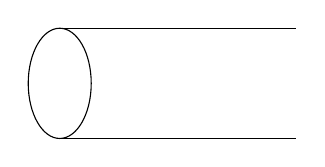
\begin{tikzpicture}
\draw (0,0) ellipse (0.4 and 0.7);
\draw (0,-0.7) -- (3,-0.7);
\draw (0,0.7) -- (3,0.7);
\end{tikzpicture}

In cylindrical coordinates, 
\begin{equation*}
\begin{aligned}
\nabla^2 \psi = \frac{1}{r} \frac{\partial}{\partial r}\left(r \frac{\partial \psi}{\partial r}\right) + \frac{1}{r^2} \frac{\partial^2 \psi}{\partial \theta^2} + \frac{\partial^2 \psi}{\partial z^2} = 0
\end{aligned}
\end{equation*}
so once again, look for a solution of the form
\begin{equation*}
\begin{aligned}
\psi\left(r,\theta,z\right) = R\left(r\right)\Theta\left(\theta\right) Z\left(z\right)\\
\implies \left(\frac{R''}{R} + \frac{1}{r} \frac{R'}{R}\right) + \frac{1}{r^2} \frac{\Theta''}{\Theta} + \frac{Z''}{Z} = 0
\end{aligned}
\end{equation*}
This implies
\begin{equation*}
\begin{aligned}
\frac{Z''}{Z} = \mu, \frac{\Theta''}{\Theta} = -\lambda, \frac{R''}{R} + \frac{1}{r}\frac{R'}{R} + \left(\mu-\frac{\lambda}{r^2}\right) = 0
\end{aligned}
\end{equation*}
For our solution to be periodic in $\theta$, we must have $\lambda = n^2$ for $n \in \N$, which implies
\begin{equation*}
\begin{aligned}
\Theta\left(\theta\right) = a_n \sin\left(n\theta\right) + b_n \cos\left(n\theta\right)
\end{aligned}
\end{equation*}
If we want our solution to decay as $z \to \infty$, we need to choose $\mu >0$ and pick the solution $Z\left(z\right) = \exp\left(-\sqrt{\mu}z\right)$.

The radial equation is \emph{Bassel's equation}. To put it in SL form, multiply through by $1/r$ to find
\begin{equation*}
\begin{aligned}
\frac{d}{dr} \left(r\frac{dR}{dr}\right) - \frac{n^2}{r} R = -\mu r R
\end{aligned}
\end{equation*}
We can rescale by introducing $x = \sqrt{\mu} r$ to obtain
\begin{equation*}
\begin{aligned}
x^2 \frac{d^2R}{dx^2} + x\frac{dR}{dx} + \left(x^2 - n^2\right) R = 0
\end{aligned}
\end{equation*}
which is independent of the eigenvalue $\mu$. This second order ODE has 2 independent solutions for each $n=0,1,2,...$, written $J_n\left(x\right)$ and $Y_n\left(x\right)$ and called \emph{Bassel functions of the first($J_n$)/second($Y_n$) kind.}

The first kind:

\begin{tikzpicture}
\draw (-.5,0) -- (5,0);
\draw (0,-.5) -- (0,1.5);
\draw (0,1) parabola[bend at end] (3,-0.5);
\draw (3,-0.5) parabola[bend at start] (4,0.3);
\end{tikzpicture}

The second kind:

\begin{tikzpicture}
\draw (-.5,0) -- (2.5,0);
\draw (0,-4) -- (0,1);
\draw (0.1,-4) parabola[bend at end] (1,0.5);
\draw (1,0.5) parabola[bend at start] (1.5,-0.3);
\end{tikzpicture}

all $J_n$ are regular at origin ($J_0\left(0\right) = 1$, $J_n\left(0\right) = 0$ for other $n$), while all $Y_n$ are singular at $x=0$.

We want $\nabla^2 \psi = 0$ inside $\Omega$, decaying to $0$ as $z \to +\infty$, regular at $r=0$ and vanishing at $r=a$. Our product ansaty(?) gives
\begin{equation*}
\begin{aligned}
\psi_{n\mu}\left(r,\theta,z\right) = \left(a_n\sin n\theta+b_n \cos n\theta\right) e^{-\sqrt{\mu}z} \left(J_n\left(\sqrt{\mu}r\right) + c_n Y_n \left(\sqrt{\mu}r\right)\right)
\end{aligned}
\end{equation*}
Regularity at $r=0$ $\implies$ $c_n=0$;\\
$\psi|_{r=a}=0$ $\implies$ $\sqrt{\mu} a = k_{in}$, where $k_{in}$ is the $i^{th}$ root of $J_n\left(x\right)$. Then
\begin{equation*}
\begin{aligned}
\psi\left(r,\theta,z\right) = \sum_{n=0}^\infty \sum_{i=1}^\infty \left(a_{ni}\sin\left(n\theta\right) + b_{ni}\cos\left(n\theta\right)\right) e^{-\frac{k_{in}z}{a}} J_n\left(k_{in}\frac{r}{a}\right)
\end{aligned}
\end{equation*}
is our general solution.

If we also impose the inhomogeneous boundary condition
\begin{equation*}
\begin{aligned}
\psi|_{z=0} = f\left(r,\theta\right)
\end{aligned}
\end{equation*}
we can fix the constants $a_{ni}$, $b_{ni}$. The Bessel functions obey the orthogonality condition
\begin{equation*}
\begin{aligned}
\int_0^a J_n\left(k_{in}\frac{r}{a}\right)J_n\left(k_{jn}\frac{r}{a}\right) r dr = \delta_{ij}\left[J'_n\left(k_{in}\right)\right]^2
\end{aligned}
\end{equation*}

e.g. At $z=0$, our solution is 
\begin{equation*}
\begin{aligned}
\psi\left(r,\theta,0\right) = \sum_{n,i}\left(a_{ni} \sin n\theta + b_{ni} \cos n\theta\right) J_n \left(k_{ni} \frac{r}{a}\right) = f\left(r,\theta\right)
\end{aligned}
\end{equation*}
This implies
\begin{equation*}
\begin{aligned}
&\underbrace{\frac{1}{\pi}\int_{-\pi}^\pi \cos  \left(m\theta\right) f\left(r,\theta\right)} = \sum_{n,i} &\underbrace{\frac{b_{ni}}{\pi} \int_{-pi}^\pi \cos \left(m\theta\right) \cos\left(n\theta\right) d\theta}& J_n \left(k_{ni} \frac{r}{a}\right)\\
&\hat{f_m}\left(r\right) &\delta_{ij}&
\end{aligned}
\end{equation*}
So
\begin{equation*}
\begin{aligned}
&\hat{f}_m\left(r\right) = \sum_i b_{mi}J_m \left(\frac{k_{mi} r}{a}\right)\\
\implies &\int_0^a J_m\left(k_{mj} \frac{r}{a}\right) \hat{f}_m\left(r\right) rdr = \frac{a^2}{2} \sum_i b_{mi}\delta_{ij} \left[J'_m \left(k_{mj} \right)\right]^2 = \frac{a^2}{2}b_{mj} \left[J'_m\left(k_{mj}\right)\right]^2\\
\implies & b_{mj} = \frac{2}{a^2 \left[J'_m \left(k_{mi}\right)\right]^2} \int_0^a J_m\left(k_{mj}\frac{r}{a}\right) \hat{f}_m \left(r\right) r dr.
\end{aligned}
\end{equation*}

\newpage

\section{The Heat Equation}

\subsection{Heat equation}

Let $\Omega \leq \R^n$ be a domain in $\R^n$, thought of as "space". The heat equation is
\begin{equation*}
\begin{aligned}
\frac{\partial \psi}{\partial t} = \kappa \nabla^2 \psi
\end{aligned}
\end{equation*}
for a function $\psi: \Omega \times \left[0,\infty\right) \to \R$ and positive constant $\kappa$, called the \emph{diffusion constant}.

The two most important properties of evolution under heat flows are:\\
$\bullet$ Total heat $\int_\Omega \psi dV$ is \emph{conserved};

\begin{proof}
\begin{equation*}
\begin{aligned}
\frac{d}{dt}\int_\Omega \psi dV = \int_\Omega \frac{\partial\psi}{\partial t} dV = \kappa \int_\Omega \left(\nabla^2\psi\right) dV = \kappa \int_{\partial\Omega} \mathbf{n} \cdot \left(\nabla \psi\right) dS
\end{aligned}
\end{equation*}
So provided $\mathbf{n} \cdot \nabla \psi = 0$, which says heat doesn't flow out of $\Omega$, $\frac{d}{dt}\int_\Omega \psi dV = 0$.
\end{proof}
 
$\bullet$ Heat flow is a strongly \emph{smoothing operation};\\
Suppose $\psi$ is an eigenfunction of the Laplacian on $\Omega$ with eigenvalue $\lambda$ (i.e. $\nabla^2 \psi = -\lambda \psi$), and $\psi = 0$ or $\mathbf{n}\cdot \nabla\psi = 0$ on $\partial \Omega$. These eigenvalues are necessarily non-negative.

\begin{proof}
\begin{equation*}
\begin{aligned}
&-\lambda \int_\Omega \psi^* \psi dV = \int_\Omega \psi^* \nabla^2 \psi dV = -\int_\Omega \nabla\psi^* \cdot \nabla\psi dV = - ||\nabla\psi||^2 \leq 0\\
\implies & \lambda = \frac{\int_\Omega \nabla \psi^* \cdot \nabla \psi dV}{\int_\Omega \left|\psi\right|^2 dV} \geq 0
\end{aligned}
\end{equation*}
we've used our boundary condition above.\\
Formally, we have that our solution to the heat equation can be written as
\begin{equation*}
\begin{aligned}
\psi\left(\mathbf{x},t\right) = \left(e^{t\nabla^2}\right)\psi\left(\mathbf{x},0\right)
\end{aligned}
\end{equation*}
(set $\kappa = 1$). Here we think $e^{t\nabla^2}$ as the Taylor expansion:
\begin{equation*}
\begin{aligned}
e^{t\nabla^2} = 1+t\nabla^2 + \frac{t^2}{2} \nabla^2\nabla^2+...
\end{aligned}
\end{equation*}
Expanding our initial data $\psi\left(\mathbf{x},0\right)$ in terms of a complete set $\left\{\psi_I\left(\mathbf{x}\right)\right\}$ of eigenfunctions of $\nabla^2$ as 
\begin{equation*}
\begin{aligned}
\psi\left(\mathbf{x},0\right) = \sum_I c_I \psi_I \left(\mathbf{x}\right)
\end{aligned}
\end{equation*}
Then we get
\begin{equation*}
\begin{aligned}
\psi\left(\mathbf{x},t\right) = e^{t\nabla^2} \left(\sum_I c_I\psi_I\left(\mathbf{x}\right)\right) = \sum_I c_I \left(e^{t\nabla^2} \psi_I\right) = \sum_I c_I e^{-\lambda_I t} \psi_I\left(\mathbf{x}\right)
\end{aligned}
\end{equation*}
We've seen (for Fourier series - true for any expansion in eigenfunctions) that the smoothness of the original function is reflected in the decay of the coefficients in the expansion as $|I| \to \infty$. Heat flow exponentially suppresses eigenfunction with large $\lambda_I$. Heat flow exponentially suppresses eigenfunction with large $\lambda_I$.
\end{proof}

The heat equation also has some symmetries:\\
If $\phi\left(x,t\right)$ obeys $$\frac{\partial \phi}{\partial t} = k\nabla^2 \phi$$ then so too does:\\
$\bullet$ $\xi\left(x,t\right) = \phi\left(x-x_0,t-t_0\right)$ -- translation in space/time;\\
$\bullet$ $\psi\left(x,t\right) = \lambda^p \phi\left(\sqrt{\lambda}x,\lambda t\right)$ rescaling by $\lambda \in \R^+$.

In particular, we can look for a \emph{similarity solution}, which is one that is independent of this scaling (up to an overall factor). i.e.
\begin{equation*}
\begin{aligned}
\psi\left(x,t\right) = \phi\left(x,t\right) = \lambda^p \phi\left(\sqrt{\lambda}x,\lambda t\right)
\end{aligned}
\end{equation*}

If this is so, then since $\phi\left(x,t\right)$ is independent of $\lambda$, we can set $\lambda$ to be anything convenient, e.g. $\lambda = \frac{1}{t}$. Then
\begin{equation*}
\begin{aligned}
\phi\left(x,t\right) = t^{-p} \phi\left(\frac{x}{\sqrt{t}},1\right) = t^{-p} u\left(\eta\right)
\end{aligned}
\end{equation*}
where $\eta = \frac{x}{\sqrt{t}}$ is the \emph{similarity variable}. Then

\begin{equation*}
\begin{aligned}
&\partial_t \phi = -pt^{p-1} u + t^{-p} \frac{\partial \eta}{\partial t} u' = t^{-p-1} \left(-pu+\eta u'\right)\\
\implies & \kappa \partial_x^2 \phi = \kappa t^{-p} \frac{\partial}{\partial x}\left(\frac{\partial \eta}{\partial x} u'\right) = \kappa t^{-p-1} u''
\end{aligned}
\end{equation*}

so the heat equation becomes an ODE for $u\left(\eta\right)$:
\begin{equation*}
\begin{aligned}
0=t^{-p-1} \left(-pu-\frac{\eta u'}{2} - \kappa u''\right)
\end{aligned}
\end{equation*}

For example, choosing $p = \frac{1}{2}$, we get
\begin{equation*}
\begin{aligned}
0 = ku'' + \frac{1}{2}\left(\eta u' + u\right) = \left(\kappa u' + \frac{\eta u}{2}\right)'
\end{aligned}
\end{equation*}

If we impose the initial condition
\begin{equation*}
\begin{aligned}
u'\left(0\right) = 0
\end{aligned}
\end{equation*}
then
\begin{equation*}
\begin{aligned}
\frac{u'}{u} = -\frac{\eta}{2\kappa}
\end{aligned}
\end{equation*}
and so
\begin{equation*}
\begin{aligned}
u\left(\eta\right) = A e^{-\eta^2/4\kappa}
\end{aligned}
\end{equation*}
therefore
\begin{equation*}
\begin{aligned}
\phi\left(x,t\right) = \frac{1}{\sqrt{4\pi t}} e^{-\frac{x^2}{4\kappa t}}
\end{aligned}
\end{equation*}
where we fixed $A$ by $\int_R \phi\left(x,t\right) dx = 1$.

This is a Gaussian with variance proportional to $t$, and is the \emph{fundamental solution} to the heat equation.

For heat flow on $\R^n \times \left[0,\infty\right)$, we'd instead get the fundamental solution
\begin{equation*}
\begin{aligned}
\phi\left(\mathbf{x},t\right) = \frac{1}{\left(4\pi \kappa t\right)^{n/2}} e^{-\frac{|\mathbf{x}|^2}{4\kappa t}}
\end{aligned}
\end{equation*}

\begin{tikzpicture}
\draw (-3,0) -- (3,0);
\draw (0,-0.5) -- (0,3);
\draw[red] (-3,0.1) .. controls (-0.8,0.3) and (-0.3,1.5) .. (0,1.5);
\draw[red] (3,0.1) .. controls (0.8,0.3) and (0.3,1.5) .. (0,1.5);
\draw[green] (-3,0.025) .. controls (-0.8,0.075) and (-0.3,0.375) .. (0,0.375);
\draw[green] (3,0.025) .. controls (0.8,0.075) and (0.3,0.375) .. (0,0.375);
\end{tikzpicture}

The fact that heat \emph{always} flows from hot to cold is apparently in conflict with the time reversibility of Newton's laws.

Einstein realised that this could be explained statistically: suppose a particle is being jostled at random s.t. the probability it moves through distance $y$ in time $\Delta t$ is $p\left(y\right)$. Assume:\\
$\bullet$ $p\left(y\right)$ independent of $t$;\\
$\bullet$ $p\left(y\right)$ is strongly peaked near $0$,\\
$\bullet$ $p\left(-y\right) = p\left(y\right)$ no preferred direction.
Let $P\left(x,t\right)$ be the probability our particle is found at $x$ at time $t$. Then
\begin{equation*}
\begin{aligned}
P\left(x,t + \Delta t\right) &= \int_{-\infty}^\infty p\left(y\right) P\left(x-y,t\right) dy\\
&\approx \int_{-\infty}^\infty \sum_{n=0}^\infty \frac{p\left(y\right)}{n!} \frac{\partial^n P}{\partial y^n} \left(x,t\right)\left(-y\right)^n dy\\
&= \sum_{n=0}^\infty \frac{\partial^n P}{\partial y^n} \frac{1}{n!} \left<y^n\right>
\end{aligned}
\end{equation*}
where $\left<y^n\right> = \int_{-\infty}^\infty p\left(y\right) y^n$. The above is then approximately
\begin{equation*}
\begin{aligned}
P\left(x,t\right) + \frac{\left<y^2\right>}{2} \frac{\partial^2 P}{\partial x^2}
\end{aligned}
\end{equation*}
with some small corrections. Then
\begin{equation*}
\begin{aligned}
\frac{P\left(x,t+\Delta t\right) - P\left(x,t\right)}{\Delta t} = \kappa \frac{\partial^2 P}{\partial x^2}
\end{aligned}
\end{equation*}
where
\begin{equation*}
\begin{aligned}
\kappa = \frac{\left<y^2\right>}{2\Delta t}
\end{aligned}
\end{equation*}
As $\Delta t$ becomes small (but still large compared to collision times) we have the heat equation.

\begin{tikzpicture}
\begin{axis} [axis lines = middle, xmin = -5,xmax = 5, ymin = -5,ymax = 5]
\addplot{x^2};
\end{axis}
\end{tikzpicture}

\subsection{Heat flow in a semi-infinite region}

Suppose $\phi\left(x,t\right)$ obeys the heat equation inside $\Omega \times\left[0,\infty\right)$ with $\Omega = \left\{x \geq 0\right\}$ subject to the boundary conditions $\phi\left(x,t\right) \to c$ as $x \to + \infty$ and
\begin{equation*}
\begin{aligned}
\phi\left(0,t\right) = \phi_0 + A\cos \left(\frac{2\pi t}{t_0}\right) + B \cos \left(\frac{2\pi t}{t_0}\right)
\end{aligned}
\end{equation*}

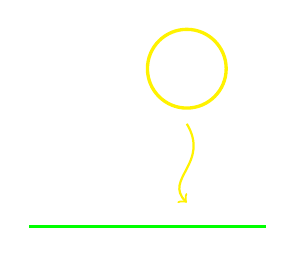
\begin{tikzpicture}
\draw[green,very thick] (0,0) -- (3,0);
\draw[yellow,very thick] (2,2.0) circle [radius=0.5cm];
\draw[yellow,thick,->] (2,1.3) .. controls (2.3,0.8) and (1.7,0.6) .. (2,0.3);
\end{tikzpicture}

To solve, we look for a simple solution to the heat equation of the form
\begin{equation*}
\begin{aligned}
\phi\left(x,t\right) = X\left(x\right) T\left(t\right)
\end{aligned}
\end{equation*}
\begin{equation*}
\begin{aligned}
\frac{T'}{T} = \kappa \frac{X''}{X} = \lambda
\end{aligned}
\end{equation*}
we want oscillatory solutions in time, so set $\lambda = i\omega$, we get
\begin{equation*}
\begin{aligned}
\phi_\omega\left(x,t\right) = e^{i\omega t} \left(a_\omega e^{-x\sqrt{\frac{i\omega}{\kappa}}} + b_\omega e^{+x \sqrt{\frac{i\omega}{\kappa}}} \right)
\end{aligned}
\end{equation*}

\begin{equation*}
\begin{aligned}
\sqrt{i\omega} = \left\{
\begin{array}{ll}
\frac{1+i}{\sqrt{2}}\sqrt{|\omega|} & \omega > 0\\
\frac{i-1}{\sqrt{2}}\sqrt{|\omega|} & \omega < 0
\end{array}
\right.
\end{aligned}
\end{equation*}

So
\begin{equation*}
\begin{aligned}
\phi\left(0,t\right) = \phi_0 + \frac{A}{2}\left(e^{i\omega_D t} + e^{-i\omega_D t}\right) + \frac{B}{2}\left(e^{i\omega_Y t} + e^{-i\omega_Y t}\right)
\end{aligned}
\end{equation*}
where
\begin{equation*}
\begin{aligned}
\omega_{D,Y} = \frac{1}{2\pi t_{D,Y}}
\end{aligned}
\end{equation*}

So we have non-zero contributions when the separation constant, $\omega = \pm \omega_D,\pm\omega_Y,0$,
\begin{equation*}
\begin{aligned}
\phi\left(x,t\right) = \phi_0 + Ae^{-\sqrt{\frac{\omega_D}{2\kappa}}x} \cos\left(\omega_D t-\sqrt{\frac{\omega_D}{2\kappa}} x\right) + Be^{-\sqrt{\frac{\omega_Y}{2\kappa}}x} \cos\left(\omega_Y t-\sqrt{\frac{\omega_Y}{2\kappa}} x\right)
\end{aligned}
\end{equation*}

Let $\Omega = \left\{\left(r,\theta,\phi\right) \in \R^3 \mid r \leq a \right\}$ and suppose $\psi:\Omega \times \left[0,\infty\right) \to \R$ obeys $\frac{\partial \psi}{\partial t} = \kappa \nabla^2 \psi$. For simplicity, we'll take $\psi\left(r,\theta,\phi\right) = \psi\left(r\right)$. We impose\\
$\bullet$ boundary condition $\psi|_{\partial \Omega \times \left(0,\infty\right)} = \psi\left(a\right) = 0$;\\
$\bullet$ initial condition $\psi|_{\Omega\times\left\{0\right\}} = \psi_0$ constant.

Look for a solution of the form $\psi\left(r,t\right) = R\left(r\right) T\left(t\right)$. Then
\begin{equation*}
\begin{aligned}
\frac{1}{\kappa T} \frac{dT}{dt} = \frac{1}{Rr^2} \frac{d}{dr}\left(r^2 \frac{dR}{dr}\right) = -\lambda^2
\end{aligned}
\end{equation*}
for some constant $\lambda$.

The radial equation is
\begin{equation*}
\begin{aligned}
\frac{d}{dr}\left(r^2 \frac{dR}{dr}\right) = -\lambda^2 r^2 R
\end{aligned}
\end{equation*}
and has solutions
\begin{equation*}
\begin{aligned}
R\left(r\right) = A_\lambda \frac{\sin\left(\lambda r\right)}{r} + B_\lambda \frac{\cos\left(\lambda r\right)}{r}
\end{aligned}
\end{equation*}

Regularity at $r=0$ forces us to set $B_\lambda = 0$, while the boundary condition $\psi_{r=a} = 0$ fixes $\lambda = \frac{n\pi}{a}$ for some $n=1,2,...$.

So our separates solution is
\begin{equation*}
\begin{aligned}
\psi_n\left(r,t\right) = \frac{A_n}{r}\sin\left(\frac{n\pi r}{a}\right) \exp \left(-\frac{n^2 \pi^2 \kappa t}{a^2}\right)
\end{aligned}
\end{equation*}
which implies that the general solution obeying homogeneous boundary condition is
\begin{equation*}
\begin{aligned}
\sum_{n \in \Z^+} \frac{A_n}{r}\sin\left(\frac{n\pi r}{a}\right) \exp\left(-\frac{n^2 \pi^2 \kappa t}{a^2}\right)
\end{aligned}
\end{equation*}
we fix the $A_n$ by imposing $\psi\left(r,0\right) = \psi_0$. So
\begin{equation*}
\begin{aligned}
&r\psi_0 = \sum_{n \in \Z^+} A_n \sin\left(\frac{n\pi r}{a}\right)\\
\implies & A_m = \frac{\psi_0}{2a}\int_0^a r\sin\left(\frac{m\pi r}{a}\right) dr = \frac{\left(-1\right)^{m+1} \psi_0}{2\pi n}
\end{aligned}
\end{equation*}
Therefore
\begin{equation*}
\begin{aligned}
\psi\left(r,t\right) = \frac{\psi_0}{2\pi r}\sum_{n \in \Z^+} \frac{\left(-1\right)^{n+1}}{n} \sin\left(\frac{n\pi r}{a}\right) \exp\left(-\frac{n^2 \pi^2 \kappa t}{a^2}\right)
\end{aligned}
\end{equation*}

Consider
\begin{equation*}
\begin{aligned}
\frac{\partial \psi}{\partial r}|_{r=a} &= -\frac{\psi_0}{a} \sum_{n \in \Z^+} \exp\left(-\frac{n^2 \pi^2 \kappa t}{a^2}\right)\\
&\approx -\frac{\psi_0}{2a} \int_{-\infty}^\infty \exp\left(-\frac{-x^2\pi^2 \kappa t}{a^2}\right) dx\\
&\approx -\frac{\psi_0}{2} \sqrt{\frac{a^2}{\pi \kappa t}}
\end{aligned}
\end{equation*}

So $$t_{now} = \frac{\psi_0^2 a^2}{\left(\frac{\partial \psi}{\partial r}\right)_{now}^2 4\kappa \pi}$$

We have $\psi_0 \sim 1000 ^\circ$C, $\frac{\partial \psi}{\partial r}|_{now} \sim 20^\circ$C$/100$m, $\kappa$ is the thermal diffusivity of rock. Then we get $t_{now} \approx 100$ million years. However we didn't take heat generated by radioactivity into account.

\newpage

\section{The Wave Equation}

\subsection{The Wave Equation}
\begin{equation*}
\begin{aligned}
\psi: \Omega \times \R \to \R
\end{aligned}
\end{equation*}
solves the wave equation if 
\begin{equation*}
\begin{aligned}
\frac{1}{c^2}\frac{\partial^2 \phi}{\partial t^2} = \nabla^2 \phi
\end{aligned}
\end{equation*}

There's a unique solution subject to \\
$\bullet$ initial conditions:
\begin{equation*}
\begin{aligned}
\psi\left(\mathbf{x},0\right) = f\left(\mathbf{x}\right)\\
\partial_t \phi\left(\mathbf{x},0\right) = g\left(\mathbf{x}\right)
\end{aligned}
\end{equation*}
$\bullet$ boundary conditions:
\begin{equation*}
\begin{aligned}
\psi\left(\mathbf{x},t\right)|_{\partial \Omega} = h\left(\mathbf{x},t\right)
\end{aligned}
\end{equation*}
which is a Dirichlet boundary condition.
\begin{proof}
We consider the \emph{energy}
\begin{equation*}
\begin{aligned}
E_\phi = \frac{1}{2} \int_\Omega \left(\frac{\partial \phi}{\partial t}\right)^2 + c^2 \left(\nabla \phi\right)\cdot\left(\nabla\phi\right)dV
\end{aligned}
\end{equation*}
Differentiating under the integral, we have
\begin{equation*}
\begin{aligned}
\frac{dE_\phi}{dt} &= \int_\Omega \frac{\partial \phi}{\partial t}\frac{\partial^2\phi}{\partial t^2} + c^2\left(\nabla\phi\right)\cdot\nabla\left(\frac{\partial \phi}{\partial t}\right) dV\\
&= \int_\Omega \frac{\partial \phi}{\partial t}\left(\frac{\partial^2 \phi}{\partial t^2} - c^2 \nabla^2 \phi\right) dV + c^2 \int_{\partial \Omega} \frac{\partial \phi}{\partial t}\left(\nabla\phi\right)\cdot\mathbf{\hat{n}} dS
\end{aligned}
\end{equation*}
where $\mathbf{\hat{n}}$ is the outward-pointing normal. Then
\begin{equation*}
\begin{aligned}
\frac{dE_\phi}{dt} = c^2 \int_{\partial \Omega} \frac{\partial \phi}{\partial t} \left(\nabla\phi\right)\cdot\mathbf{\hat{n}} dS
\end{aligned}
\end{equation*}
So $E_\phi$ is constant in time if no energy flows out of the region $\Omega$ (i.e. if this boundary term vanished).

So let $\phi_1,\phi_2$ each solve the wave equation with the same boundary conditions and initial conditions. Then $\delta\phi = \phi_2 - \phi_1$ obeys the wave equation with
\begin{equation*}
\begin{aligned}
\delta_\phi|_{\partial \Omega \times \R} = 0,\\
\delta\phi|_{\Omega\times\left\{0\right\}} = 0,\\
\partial_t \left(\delta\phi\right)|_{\Omega \times \left\{0\right\}} = 0
\end{aligned}
\end{equation*}
That implies 
\begin{equation*}
\begin{aligned}
\frac{dE_{\delta\phi}}{dt} = \int_\Omega \partial_t \left(\delta\phi\right) \mathbf{\hat{n}}\cdot\nabla\delta\phi dS = 0
\end{aligned}
\end{equation*}
since $\partial_t \left(\delta \phi\right)|_{\partial \Omega} = 0$. So
\begin{equation*}
\begin{aligned}
E_{\delta\phi}\left(t\right) = E_{\delta_\phi}\left(0\right) = 0
\end{aligned}
\end{equation*}
since $\delta\phi|_{\Omega\times\left\{0\right\}} = \partial_t \delta\phi|_{\Omega\times\left\{0\right\}} = 0$.\\
However, $E_{\delta\phi}$ is the integral of non-negative quantities, so $E_{\delta\phi} = 0$ if and only if $\frac{\partial\delta\phi}{\partial t} = 0$ and $\nabla\left(\delta\phi\right) = 0$ $\forall \left(\mathbf{x},t\right) \in \Omega\times \R$ (at best if $\delta \phi$ continuous).\\
So $\delta\phi = 0$ always, so $\phi_1 = \phi_2$.
\end{proof}

\begin{eg}
Consider a string of undisturbed length $L$:

\begin{tikzpicture}
\draw (0,0) .. controls (0.5,1) and (1.5,-1) .. (2,0);
\draw (2,0) .. controls (3,1) and (3.5,-0.2) .. (4,0);
\end{tikzpicture}

(see figure 1)

And let $T_A$, $T_B$ be tensions pulling tangentially. The string makes no lateral displacement. That means
\begin{equation*}
\begin{aligned}
T_A \cos \theta_A = T_B \cos \theta_B = T
\end{aligned}
\end{equation*}
Newton's 2nd law gives
\begin{equation*}
\begin{aligned}
\mu \delta x \frac{\partial^2 \phi}{\partial t^2} = T_B \sin \theta_B - T_A \sin \theta_A\\
\implies \frac{\mu\delta x}{T} \frac{\partial^2 \phi}{\partial t^2} &= \frac{T_B \sin \theta_B}{T_B \cos\theta_B} - \frac{T_A \sin \theta_A}{T_A \cos \theta_A} \\&= \tan \theta_B - \tan \theta_A\\
&= \frac{\partial \phi}{\partial x}|_B - \frac{\partial \phi}{\partial x}|_A\\
&\approx \frac{\partial^2 \phi}{\partial x^2} \delta x
\end{aligned}
\end{equation*}
So $\phi$ obeys
\begin{equation*}
\begin{aligned}
\frac{1}{c^2}\frac{\partial^2\phi}{\partial t^2} = \frac{\partial^2 \phi}{\partial x^2}
\end{aligned}
\end{equation*}
with
\begin{equation*}
\begin{aligned}
c^2 = \frac{T}{\mu}
\end{aligned}
\end{equation*}
as well as initial conditions
\begin{equation*}
\begin{aligned}
\phi\left(x,0\right) = f\left(x\right),\\
\partial_t \phi\left(x,0\right) = g\left(x\right)
\end{aligned}
\end{equation*}
and boundary conditions
\begin{equation*}
\begin{aligned}
\phi\left(0,t\right) = \phi\left(L,t\right) = 0
\end{aligned}
\end{equation*}

We look for a solution of the form $\phi\left(x,t\right) = X\left(x\right)T\left(t\right)$. Then
\begin{equation*}
\begin{aligned}
X'' = -\lambda^2 X,\\
T'' = -c^2 \lambda^2 T
\end{aligned}
\end{equation*}
For $X$ we have
\begin{equation*}
\begin{aligned}
A\sin\left(\lambda x\right) + B\cos\left(\lambda x\right)
\end{aligned}
\end{equation*}
By boundary condition, $B=0$. So the solutions are
\begin{equation*}
\begin{aligned}
\phi_n\left(x,t\right) = \sin\left(n\pi x/L\right) \left[A_n \sin\left(n\pi ct/L\right) + B_n \cos\left(n\pi ct/L\right)\right]
\end{aligned}
\end{equation*}
The general solution obeying homogeneous boundary conditions is
\begin{equation*}
\begin{aligned}
\phi\left(x,t\right) = \sum_{n=1}^\infty \sin\left(n\pi x/L\right) \left[A_n \sin\left(n\pi ct/L\right) + B_n \cos\left(n\pi ct/L\right)\right]
\end{aligned}
\end{equation*}

The coefficients $A_n$, $B_n$ are fixed by the initial conditions on $\phi$, $\partial_t \phi$ respectively. We find
\begin{equation*}
\begin{aligned}
B_n = \frac{2}{L} \int_0^L f\left(x\right) \sin\left(n\pi x/L\right) dx,\\
A_n = \frac{2}{n\pi c}\int_0^L g\left(x\right) \sin\left(n\pi x/L\right) dx
\end{aligned}
\end{equation*}
\end{eg}

\begin{eg}
Suppose we pluck the string so that at $t=0$,
\begin{equation*}
\begin{aligned}
f\left(x\right) = \left\{\begin{array}{ll}
\frac{2hx}{L} & 0\leq x \leq \frac{L}{2}\\
\frac{2h\left(L-x\right)}{L} & \frac{L}{2} \leq x \leq L
\end{array}
\right.
\end{aligned}
\end{equation*}

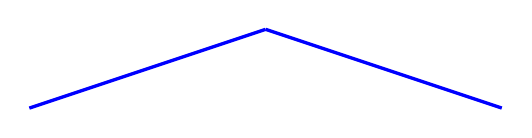
\begin{tikzpicture}
\draw[very thick,blue] (0,0) -- (3,1);
\draw[very thick,blue] (3,1) -- (6,0);
\end{tikzpicture}

release from rest: $g\left(x\right) = 0$.

Then the Fourier coefficients are
\begin{equation*}
\begin{aligned}
\hat{f}_n \left\{ \begin{array}{ll}
\left(-1\right)^{\left(n+1\right)/2} \frac{8h}{n^2 \pi^2} & n \text{ odd}\\
0 & n \text{ even}
\end{array}
\right.
\end{aligned}
\end{equation*}
So
\begin{equation*}
\begin{aligned}
\phi\left(x,t\right) = \frac{8h}{\pi^2} \sum_{m=1}^\infty \frac{\left(-1\right)^{m+1}}{\left(2m-1\right)^2} \sin\frac{\left(2m-1\right)\pi x}{L} \cos\frac{\left(2m-1\right) \pi c t}{L}
\end{aligned}
\end{equation*}

Note that all the frequencies of the different normal modes $\phi_n\left(x,t\right)$ are integer multiples of the fundamental frequency $\pi c/L$.

The kinetic energy of the string (mass/unit length $\mu$) is
\begin{equation*}
\begin{aligned}
KE = \frac{1}{2}\mu \int_0^L \left(\frac{\partial \phi}{\partial t}\right)^2 dx
\end{aligned}
\end{equation*}

Because the string is under tension, it also has potential energy. For a small piece of the string, the extension is $\delta s - \delta x$, where $\delta x$ is the original length (difference in the $x$ direction) and $\delta s$ is the strength under tension. We have
\begin{equation*}
\begin{aligned}
\delta s \approx \sqrt{\delta \phi^2 + \delta x^2}
\end{aligned}
\end{equation*}
so the PE of this piece is
\begin{equation*}
\begin{aligned}
T\left(\sqrt{\left(\frac{\partial \phi}{\partial x}\right)^2 +1} - 1 \right) \delta x \approx \frac{1}{2}T \left(\frac{\partial \phi}{\partial x}\right)^2
\end{aligned}
\end{equation*}
Integrating over the length of the string,
\begin{equation*}
\begin{aligned}
PE = \frac{T}{2}\int_0^L \left(\frac{\partial \phi}{\partial x}\right)^2 dx
\end{aligned}
\end{equation*}
so the total energy at time $t$ is
\begin{equation*}
\begin{aligned}
E &= KE + PE\\
&= \frac{\mu}{2} \int_0^L \left(\frac{\partial \phi}{\partial t}\right)^2 + c^2 \left(\frac{\partial \phi}{\partial x}\right)^2 dx
\end{aligned}
\end{equation*}
as before ($\mu = 1$).

Plug in our general solution, we obtain
\begin{equation*}
\begin{aligned}
KE\left(t\right) = \frac{\mu \pi^2 c^2}{4L}\sum_{n=1}^\infty n^2 \left[A_n \sin\left(\frac{n\pi ct}{L}\right) - B_n \cos\left(\frac{n\pi ct}{L}\right)\right]^2
\end{aligned}
\end{equation*}
and
\begin{equation*}
\begin{aligned}
PE\left(t\right) = \frac{\mu \pi^2 c^2}{4L}\sum_{n=1}^\infty n^2 \left[A_n \cos\left(\frac{n\pi ct}{L}\right) + B_n \sin\left(\frac{n\pi ct}{L}\right)\right]^2
\end{aligned}
\end{equation*}
So
\begin{equation*}
\begin{aligned}
E\left(t\right) = \frac{\mu c^2 \pi^2}{4L} \sum_{n=1}^\infty n^2\left(A_n^2 + B_n^2\right)
\end{aligned}
\end{equation*}
which is independent of time.

The string looks just like an infinite collection of harmonic oscillators with frequencies $n\pi c/L$. They behave independently - the solution is a \emph{sum} of terms for each $n$ separately.
\end{eg}

\subsection{Vibration of a Circular Membrane}
Let $$\Omega = \left\{ \left(r,\theta\right) \in \R^2, r\leq 1\right\}$$ and suppose
\begin{equation*}
\begin{aligned}
\phi: \Omega \times \left[0,\infty\right) \to \R
\end{aligned}
\end{equation*}
solves
\begin{equation*}
\begin{aligned}
\frac{1}{c^2}\frac{\partial^2 \phi}{\partial t^2} = \nabla^2 \phi
\end{aligned}
\end{equation*}
inside $\Omega$, with initial conditions $\phi\left(r,\theta,0\right) = f\left(r,\theta\right)$, $\partial_t\phi\left(r,0,0\right) = f\left(r,\theta\right)$ and boundary condition $\phi\left(1,\theta,t\right) = 0$.

Let $\phi\left(r,\theta,t\right) = R\left(r\right)\Theta\left(\theta\right)T\left(t\right)$. Then
\begin{equation*}
\begin{aligned}
T'' = -c^2 \lambda T, \Theta'' = -\mu \Theta, r\left(rR'\right)' + \left(r^2 \lambda - \mu\right) R = 0
\end{aligned}
\end{equation*}

We want the solution to be periodic in $\theta$, so choose $\mu = m^2$ for some $n \in \N$. The radial equation is then
\begin{equation*}
\begin{aligned}
r\left(rR'\right) + \left(r^2\lambda - m^2\right)R = 0
\end{aligned}
\end{equation*}
which is the Bessel's equation of order $m$. So
\begin{equation*}
\begin{aligned}
R\left(r\right) = a_m J_m \left(\sqrt{\lambda} r \right) + b_m Y_m \left(\sqrt{\lambda} r\right)
\end{aligned}
\end{equation*}

To obey boundary conditions at $r=1$, we must choose $\sqrt{\lambda}$ to be a root $k_{mi}$ of the $m^{th}$ order Bessel function. So
\begin{equation*}
\begin{aligned}
T\left(t\right) = A_{mi}\sin\left(k_{mi} ct\right) + C_{mi} \cos\left(k_{mi} ct\right)
\end{aligned}
\end{equation*}

Combining all the terms, we have a \emph{horrible} solution:
\begin{equation*}
\begin{aligned}
\phi\left(r,\theta,t\right) = &\sum_{i=1}^\infty \left[A_{0i} \sin \left(k_{0i} ct\right) + C_{0i} \cos\left(k_{0i} ct\right)\right] J_0 \left(k_{0i} r\right) 
\\& +\sum_{m=1}^\infty \sum_{i=1}^\infty \left[A_{mi} \cos\left(m\theta\right) + B_{mi}\sin \left(m\theta\right)\right] \sin\left(k_{mi} ct\right) J_m\left(k_{mi} r\right) 
\\&+\sum_{m=1}^\infty \sum_{i=1}^\infty \left[C_{mi} \cos\left(m\theta\right) + D_{mi} \sin\left(m\theta\right)\right] \cos\left(k_{mi} ct\right) J_m \left(k_{mi} r\right)
\end{aligned}
\end{equation*}
The coefficients $\left\{A,B,C,D\right\}_{mi}$ are fixed by the inhomogeneous conditions.

\begin{eg}
If a drum is initially flat ($\phi|_{t=0} = 0$), but struck in the centre so that $\partial_t\phi|_{t=0} \ g\left(r\right)$, then there is no angular dependence, so only the $m=0$ terms survive, and $C_{0i} = 0$. So
\begin{equation*}
\begin{aligned}
\phi\left(r,\theta,t\right) = \sum_{i=1}^\infty A_{0i} \sin\left(k_{0i} ct\right) J_0 \left(k_{0i} r\right)
\end{aligned}
\end{equation*}
where (as an exercise)
\begin{equation*}
\begin{aligned}
A_{0i} = \frac{2}{ck_{0i}} \frac{1}{\left[J'_0\left(k_{0i}\right)\right]^2} \int_0^1 J_0 \left(k_{0i}r\right) g\left(r\right) r dr
\end{aligned}
\end{equation*}
\end{eg}

\begin{tikzpicture}
\draw (-1,3) .. controls (1,3) .. (1,1) ..
 controls (2,1) .. (2,-1) ..
  controls (1,-1) .. (1,-3) ..
   controls (-1,-3) .. (-1,-1) ..
    controls (-2,-1) .. (-2,1) .. 
    controls (-1,1) .. cycle;
    node [centre]($\Omega$)
\end{tikzpicture}

In general there can be strange frequencies depending on $\Omega$. There is an interesting question -- if we can 'hear' the shape of a drum. The answer is no (the first example with $\dim\left(\Omega\right) = 16$ and now a lot of examples)!

But if $\Omega$ is convex then the answer is yes.

Also, let $N\left(\lambda_0\right)$ be the number of eigenvalues of $\nabla^2|_\Omega$ that is less than $\lambda_0$. Then
\begin{equation*}
\begin{aligned}
Area\left(\Omega\right) = \lim_{\lambda_0\to\infty} \frac{N\left(\lambda_0\right)}{\lambda_0} 4\pi^2
\end{aligned}
\end{equation*}
(by Weyl). We can also get limits on Perimeter($\Omega)$ (c.f. Spectral geometry in Part III).

\end{document}